\chapter{Phương pháp đề xuất}
\section{Kiến trúc tổng thể}

Hệ thống được thiết kế linh hoạt để tiếp nhận đầu vào đa dạng, cho phép người dùng tìm kiếm thông qua các câu truy vấn văn bản hoặc tải lên hình ảnh trực tiếp. Dựa trên những dữ liệu đầu vào này, hệ thống sẽ phân tích và đề xuất các sản phẩm chất lượng cao, đảm bảo sự tương thích sát sao nhất với nhu cầu và sở thích cá nhân của từng người dùng. Để hiện thực hóa điều này, nhóm sử dụng bộ dữ liệu Amazon Reviews làm nền tảng huấn luyện. Đây là một tập dữ liệu phong phú bao gồm các đặc trưng từ phía người dùng như nội dung đánh giá, điểm xếp hạng, và mức độ hữu ích của đánh giá đó, kết hợp cùng siêu dữ liệu sản phẩm item metadata như mô tả chi tiết, giá bán và hình ảnh gốc; tất cả được liên kết chặt chẽ với nhau thông qua mã định danh sản phẩm.

Về mặt phương pháp hoạt động, đồ án xây dựng một quy trình xử lý hiện đại kết hợp giữa kiến trúc Two-Tower và LLM nhằm đạt được độ chính xác cao trong việc gợi ý dựa trên hành vi mua sắm quá khứ. Phương pháp Two-Tower (hay Bi-Encoder) là một kiến trúc mạng nơ-ron tiên tiến được sử dụng rộng rãi trong các hệ thống gợi ý và tìm kiếm thông tin quy mô lớn, đóng vai trò then chốt trong giai đoạn truy xuất ứng viên. Kiến trúc này vận hành dựa trên hai nhánh mạng nơ-ron độc lập hoạt động song song: Tháp người dùng (User Tower) chịu trách nhiệm mã hóa các đặc trưng về hành vi, lịch sử và ngữ cảnh của người dùng, trong khi Tháp sản phẩm (Item Tower) xử lý các thông tin thuộc tính đa phương thức của sản phẩm như hình ảnh, văn bản mô tả hay thông số kỹ thuật. Cả hai tháp đều có nhiệm vụ chuyển đổi dữ liệu đầu vào phức tạp thành các vector embedding nén trong cùng một không gian tiềm ẩn, và mức độ phù hợp giữa người dùng và sản phẩm được xác định ở bước cuối cùng thông qua phép tính tích vô hướng hoặc độ tương đồng cosine. Ưu điểm vượt trội của Two-Tower nằm ở khả năng tách biệt quá trình tính toán, cho phép hệ thống lập chỉ mục trước hàng triệu vector sản phẩm, từ đó giải quyết bài toán tìm kiếm và gợi ý trong thời gian thực với độ trễ cực thấp mà vẫn đảm bảo nắm bắt được các mối quan hệ ngữ nghĩa sâu sắc.

\begin{figure}[H]
    \centering
    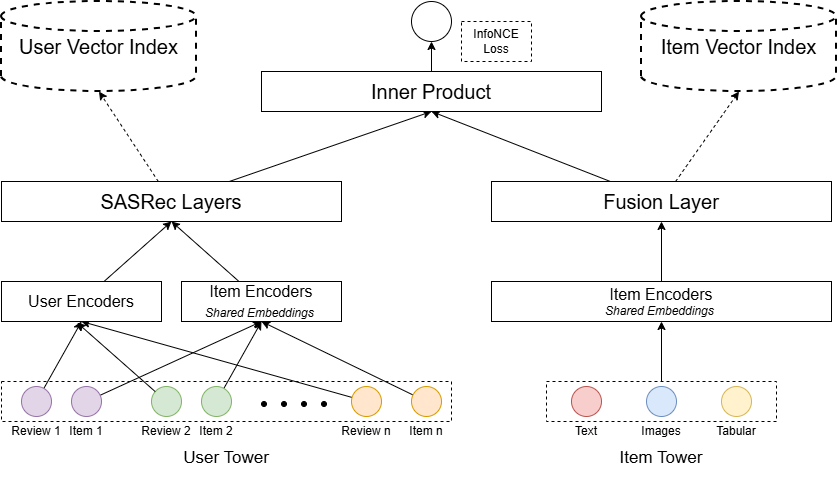
\includegraphics[width=0.8\textwidth]{Images/two_tower_model.png}
    \caption{Mô hình two-tower}
    \label{fig:overall_arch}
\end{figure}

Hình \ref{fig:overall_arch} minh họa kiến trúc tổng quát của mô hình đề xuất, được xây dựng dựa trên khung làm việc  Mạng nơ-ron Hai tháp. Mục tiêu cốt lõi của thiết kế này là tách biệt quá trình mã hóa Người dùng (User Modeling) và Sản phẩm (Item Modeling) thành hai luồng xử lý độc lập, cho phép tối ưu hóa hiệu năng trong giai đoạn truy xuất thời gian thực.

Luồng xử lý của hệ thống được chia thành hai nhánh chính:

\noindent \textbf{1. Tháp Người dùng (User Tower - Nhánh bên trái):}
Tháp này chịu trách nhiệm mô hình hóa sở thích người dùng dựa trên chuỗi lịch sử hành vi. Điểm cải tiến trong kiến trúc này là đầu vào không chỉ bao gồm định danh sản phẩm (Item ID) đơn thuần, mà là một chuỗi các cặp dữ liệu \textbf{(Review + Item)}.
\begin{itemize}
    \item Mỗi tương tác quá khứ được biểu diễn kết hợp giữa đặc trưng sản phẩm và nội dung đánh giá (Review) tương ứng, giúp mô hình nắm bắt được ngữ nghĩa và thái độ của người dùng tại thời điểm đó.
    \item Các thông tin này đi qua các bộ mã hóa User Encoders (nơi chứa khối xử lý chuỗi SASRec) và được tổng hợp tại lớp \textit{Fusion Layer} để tạo ra vector đại diện người dùng cuối cùng $\mathbf{u}$.
\end{itemize}

\noindent \textbf{2. Tháp Sản phẩm (Item Tower - Nhánh bên phải):}
Tháp này chịu trách nhiệm mã hóa các đặc trưng đa phương thức của một sản phẩm ứng viên (Candidate Item).
\begin{itemize}
    \item Đầu vào bao gồm dữ liệu văn bản (Text), hình ảnh (Images) và dữ liệu bảng (Tabular).
    \item Để đảm bảo tính nhất quán của không gian vector, hệ thống áp dụng kỹ thuật \textbf{Shared Embeddings} (Chia sẻ trọng số nhúng) cho các Item ID giữa hai tháp.
    \item Tương tự, các đặc trưng này được tổng hợp để tạo ra vector đại diện sản phẩm $\mathbf{v}$.
\end{itemize}

\noindent \textbf{3. Cơ chế Tương tác và Huấn luyện:} Hai tháp hoạt động song song và hoàn toàn không chia sẻ thông tin trong quá trình tính toán (Late Interaction). Tại lớp cuối cùng, sự tương đồng giữa người dùng và sản phẩm được tính toán thông qua tích vô hướng (Inner Product).

Mô hình được huấn luyện bằng hàm mất mát InfoNCE Loss theo nguyên lý Học tương phản. Sau khi huấn luyện, các vector người dùng và sản phẩm sẽ được lập chỉ mục vào các Cơ sở dữ liệu Vector (Vector Index) để phục vụ cho bài toán tìm kiếm láng giềng gần nhất (ANN Search).

Trên cơ sở các biểu diễn vector đặc trưng đã được trích xuất và đồng bộ hóa từ hai nhánh của mô hình, hệ thống chuyển sang giai đoạn truy xuất ứng viên thông qua cơ chế tính toán độ tương đồng trong không gian vector. Hình \ref{fig:retrieval} mô tả quá trình này.

\begin{figure}[H]
    \centering
    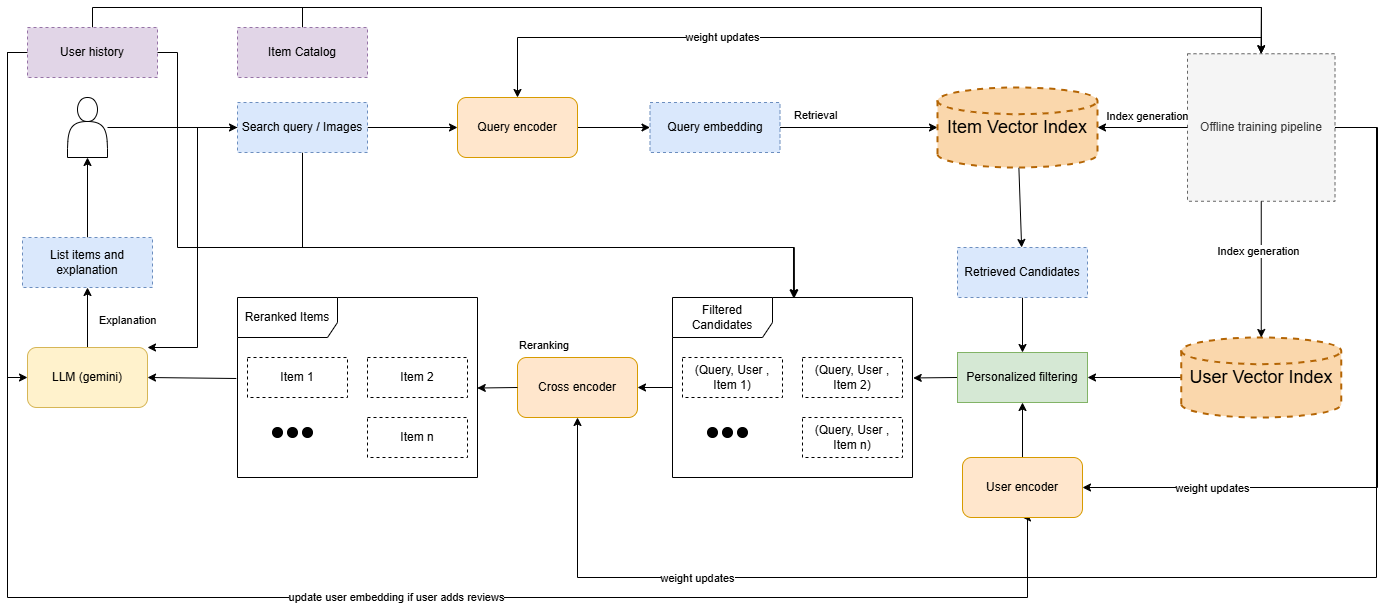
\includegraphics[width=1\textwidth]{Images/retrieval.png}
    \vspace{0.5cm}
    \caption{Quá trình Truy xuất sản phẩm}
    \label{fig:retrieval}
\end{figure}

Quy trình tìm kiếm bắt đầu khi người dùng thực hiện một truy vấn chủ động thông qua văn bản hoặc hình ảnh. Dữ liệu đầu vào này được chuyển đến bộ Query Encoders để thực hiện quá trình vector hóa. Tại đây, truy vấn thô được chuyển đổi thành vector nhúng (Query Embedding) nằm trong cùng không gian chiều với các vector sản phẩm đã được lập chỉ mục trước đó. Hệ thống sau đó sử dụng vector truy vấn này để quét qua Item Vector Index, thực hiện các phép toán tìm kiếm láng giềng gần nhất nhằm trích xuất ra tập hợp các ứng viên tiềm năng (Retrieved Candidates). Mục tiêu của giai đoạn này là tối ưu hóa độ phủ (Recall), đảm bảo thu thập được tất cả các sản phẩm có sự tương đồng về mặt ngữ nghĩa với ý định tìm kiếm của người dùng.

Điểm khác biệt của hệ thống so với các công cụ tìm kiếm truyền thống nằm ở cơ chế Personalized Filtering (Lọc cá nhân hóa). Song song với quá trình truy xuất dựa trên từ khóa, hệ thống đồng thời tham chiếu đến User Vector Index để trích xuất vector đặc trưng của người dùng—vốn được tổng hợp từ lịch sử hành vi và sở thích trong quá khứ. Vector người dùng này đóng vai trò như một bộ lọc ngữ cảnh, giúp điều chỉnh danh sách ứng viên ban đầu. Nhờ đó, các kết quả tìm kiếm không chỉ chính xác về mặt nội dung (ví dụ: đúng là "giày thể thao") mà còn phù hợp với gu thẩm mỹ riêng (ví dụ: ưu tiên "thương hiệu Nike" hay "phong cách tối giản") của từng cá nhân.

Tiếp theo, những ứng viên được lọc được đưa vào bộ Reranking để sắp xếp lại thứ hạng dựa vào query và lịch sử đánh giá của người dùng.

Sau khi danh sách ứng viên đã được sơ lọc, tập dữ liệu này được chuyển đến module LLM Reranking để thực hiện bước tinh chỉnh cuối cùng. Tại đây, một LLM sẽ phân tích sâu hơn mối quan hệ giữa truy vấn, chân dung người dùng và đặc điểm chi tiết của sản phẩm để sắp xếp lại thứ tự hiển thị. Quá trình này giúp loại bỏ các kết quả nhiễu và đưa các sản phẩm phù hợp nhất lên vị trí ưu tiên. Cuối cùng, hệ thống trả về danh sách sản phẩm kèm theo lời giải thích (List Items and explanation), giúp người dùng hiểu rõ lý do tại sao sản phẩm được đề xuất, qua đó tăng cường tính minh bạch và độ tin cậy của trải nghiệm tìm kiếm.

\section{Xây dựng Tháp Sản phẩm}

Trọng tâm của các hệ thống gợi ý hiện đại nằm ở khả năng chuyển đổi dữ liệu đa phương thức phức tạp thành các vector biểu diễn trong không gian ẩn, nơi khoảng cách hình học giữa các vector phản ánh trực tiếp mức độ tương đồng về mặt ngữ nghĩa. Trong kiến trúc đề xuất, Tháp Sản phẩm được thiết kế để xử lý song song và mã hóa ba luồng dữ liệu đặc trưng từ tập dữ liệu Amazon Reviews.

Đối với luồng \textbf{dữ liệu văn bản}, thông tin đầu vào được tổng hợp từ bốn trường dữ liệu giàu ngữ nghĩa bao gồm tiêu đề, mô tả chi tiết, đặc tính và thông số kỹ thuật của sản phẩm. Khối dữ liệu phi cấu trúc này được mã hóa thông qua mô hình ngôn ngữ BERT, cho phép hệ thống nắm bắt sâu sắc các ngữ cảnh và mối quan hệ từ vựng phức tạp mà các phương pháp nhúng từ truyền thống không thể thực hiện được.

Song song với đó, luồng \textbf{dữ liệu thị giác} tận dụng các hình ảnh sản phẩm gốc ở độ phân giải cao từ trường dữ liệu hình ảnh. Hệ thống sử dụng kiến trúc Vision Transformer (ViT) làm bộ trích xuất đặc trưng, giúp chuyển đổi các tín hiệu thị giác thành các vector đặc trưng toàn cục mang tính phân biệt cao, bổ sung thông tin trực quan quan trọng cho việc nhận diện sản phẩm.

Cuối cùng, luồng \textbf{dữ liệu dạng bảng} bao gồm các thuộc tính cấu trúc định lượng như điểm đánh giá trung bình, số lượng phản hồi, cùng các thông tin định danh phân loại như danh mục chính, danh mục phụ và thông tin cửa hàng. Các đặc trưng này được xử lý bởi một mạng nơ-ron đa tầng (MLP), có nhiệm vụ học các tương tác phi tuyến tính giữa các thuộc tính số học và phân loại. Đầu ra từ ba nhánh xử lý độc lập nêu trên sau đó được đồng bộ hóa và đi qua một tầng hợp nhất (Fusion Layer) để tạo thành một vector biểu diễn duy nhất, định hình nên bản sắc toàn diện của sản phẩm trong không gian tìm kiếm.

\begin{figure}[H]
    \centering
    % Đảm bảo tên file ảnh đúng với file bạn đã upload
    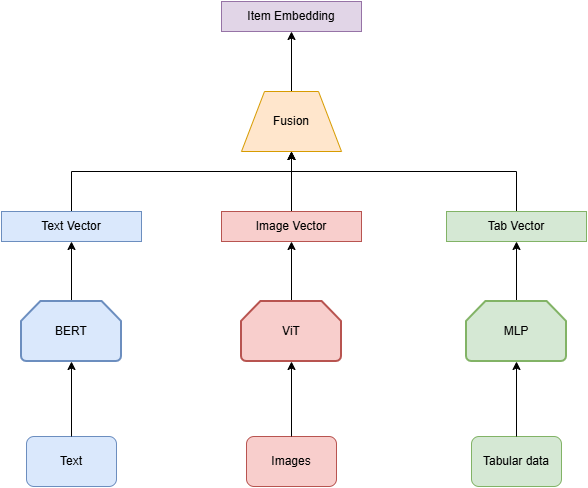
\includegraphics[width=0.8\textwidth]{Images/item_embedding.png} 
    \vspace{0.5cm}
    \caption{Kiến trúc Item Tower: Quy trình mã hóa và hợp nhất dữ liệu Đa phương thức}
    \label{fig:item_embedding}
\end{figure}

\subsection{Text Encoder: Mô-đun Mã hóa Văn bản}

TextEncoder là mô-đun mạng nơ-ron kế thừa từ \texttt{torch.nn.Module}, chịu trách nhiệm chuyển đổi dữ liệu văn bản thô (như tiêu đề, mô tả sản phẩm) thành các vector đặc trưng dày đặc (dense vectors). Đây là thành phần cốt lõi kiến tạo không gian biểu diễn ngôn ngữ cho toàn bộ kiến trúc tháp sản phẩm.

\textbf{1. Lựa chọn Mô hình và Chiến lược Huấn luyện}

Hệ thống tích hợp mô hình \texttt{all-mpnet-base-v2} làm mạng xương sống. Dựa trên bảng xếp hạng MTEB, kiến trúc MPNet thể hiện hiệu năng vượt trội trong phân khúc mô hình tầm trung \cite{6} đối với tác vụ tìm kiếm ngữ nghĩa, nhờ được huấn luyện trước trên hơn một tỷ cặp câu \cite{10}. 

Về chiến lược huấn luyện, hệ thống áp dụng cơ chế Trích xuất Đặc trưng (Feature Extraction) bằng cách đóng băng toàn bộ trọng số của khối MPNet thông qua \texttt{torch.no\_grad()}. Thiết kế này biến mô hình ngôn ngữ thành một bộ trích xuất tĩnh, giúp hệ thống tiết kiệm tối đa tài nguyên bộ nhớ GPU, đồng thời bảo toàn nguyên vẹn tri thức ngữ nghĩa gốc, tránh hiện tượng quên thảm khốc (catastrophic forgetting) khi huấn luyện trên miền dữ liệu thương mại điện tử mới.

\textbf{2. Luồng Xử lý Dữ liệu (Data Pipeline)}

Để đảm bảo hiệu năng, danh sách văn bản đầu vào được chia nhỏ thành các lô (mini-batches) và xử lý qua ba giai đoạn nối tiếp:

\begin{itemize}
    \item \textbf{Giai đoạn 1: Phân mảnh và Chuẩn bị ma trận chú ý (Tokenization):} Hệ thống sử dụng thuật toán WordPiece để phân rã câu thành các từ phụ (sub-words), giải quyết triệt để vấn đề từ vựng ngoài từ điển. Các chuỗi được đệm hoặc cắt bớt để đồng bộ chiều dài. Song song đó, một ma trận Mặt nạ chú ý được sinh ra, gán giá trị 1 cho token mang ngữ nghĩa và giá trị 0 cho token đệm, nhằm định tuyến chính xác sự tập trung của cơ chế Self-Attention.
    
    \item \textbf{Giai đoạn 2: Trích xuất đặc trưng và Masked Mean Pooling:} Chuỗi token được đưa qua khối MPNet tĩnh để sinh ra các vector ngữ cảnh. Nhằm tận dụng thông tin từ toàn bộ câu thay vì chỉ phụ thuộc vào token \texttt{[CLS]}, hệ thống áp dụng kỹ thuật Pooling trung bình có trọng số. Cụ thể, các vị trí token đệm bị triệt tiêu về 0, và vector đại diện cuối cùng được tính bằng trung bình cộng của các token thực:
    \begin{equation}
        e_{\text{pooled}} = \frac{\sum_{i=1}^{L} (h_i \cdot \text{mask}_i)}{\sum_{i=1}^{L} \text{mask}_i + \epsilon}
    \end{equation}
    Trong đó, $h_i$ là trạng thái ẩn của token thứ $i$, $\text{mask}_i$ là mặt nạ tương ứng, và $\epsilon$ là hằng số cực nhỏ ($10^{-9}$) nhằm duy trì độ ổn định số học.
    
    \item \textbf{Giai đoạn 3: Chiếu không gian và Chuẩn hóa:} Vector tổng hợp $e_{\text{pooled}}$ đi qua một tầng mạng tuyến tính (\texttt{nn.Linear}) để thực hiện phép nén không gian ẩn:
    \begin{equation}
        \mathbb{R}^{768} \rightarrow \mathbb{R}^{256}
    \end{equation}
    Phép biến đổi này đóng vai trò đồng bộ hóa kích thước đặc trưng văn bản với tháp người dùng và các luồng dữ liệu hình ảnh. Cuối cùng, vector đầu ra trải qua bước chuẩn hóa L2, đưa về dạng vector đơn vị nhằm tối ưu hóa cho hàm Contrastive Loss hoạt động dựa trên độ tương đồng Cosine.
\end{itemize}

\subsection{Image Encoder: Mô-đun Mã hóa Hình ảnh}

\texttt{ImageEncoder} chịu trách nhiệm chuyển đổi dữ liệu hình ảnh thô thành các vector đặc trưng nén. Đặc thù của sàn thương mại điện tử là một sản phẩm thường sở hữu nhiều biến thể hình ảnh (ảnh chính diện, góc cạnh, bao bì). Thay vì chọn ngẫu nhiên hoặc tính trung bình cộng đơn thuần, điểm nhấn thiết kế của mô-đun này là việc tích hợp cơ chế Gating thông minh nhằm tự động đánh giá và tổng hợp thông tin từ nhiều nguồn ảnh thành một đại diện duy nhất.

\vspace{0.3cm}
\noindent \textbf{1. Lựa chọn Mô hình và Chiến lược Huấn luyện}

Hệ thống sử dụng kiến trúc Vision Transformer (ViT), cụ thể là biến thể \texttt{vit\_base\_patch16\_224}. Mô hình này chia ảnh đầu vào thành các mảnh (\textit{patches}) kích thước $16 \times 16$ pixels để xử lý tuần tự, mang lại sự cân bằng tối ưu giữa độ chính xác và chi phí tài nguyên \cite{11}. 

Tương tự như mô đun ngôn ngữ, chiến lược Trích xuất Đặc trưng được áp dụng bằng cách đóng băng toàn bộ trọng số mạng nền (\texttt{requires\_grad = False}). Kỹ thuật này triệt tiêu chi phí tính toán gradient, đồng thời bảo toàn các đặc trưng thị giác cốt lõi đã được mạng ViT học từ tập ImageNet, tránh hiện tượng quên thảm khốc (\textit{catastrophic forgetting}).

\vspace{0.3cm}
\noindent \textbf{2. Luồng Xử lý Dữ liệu (Data Pipeline)}

\begin{figure}[H]
    \centering
    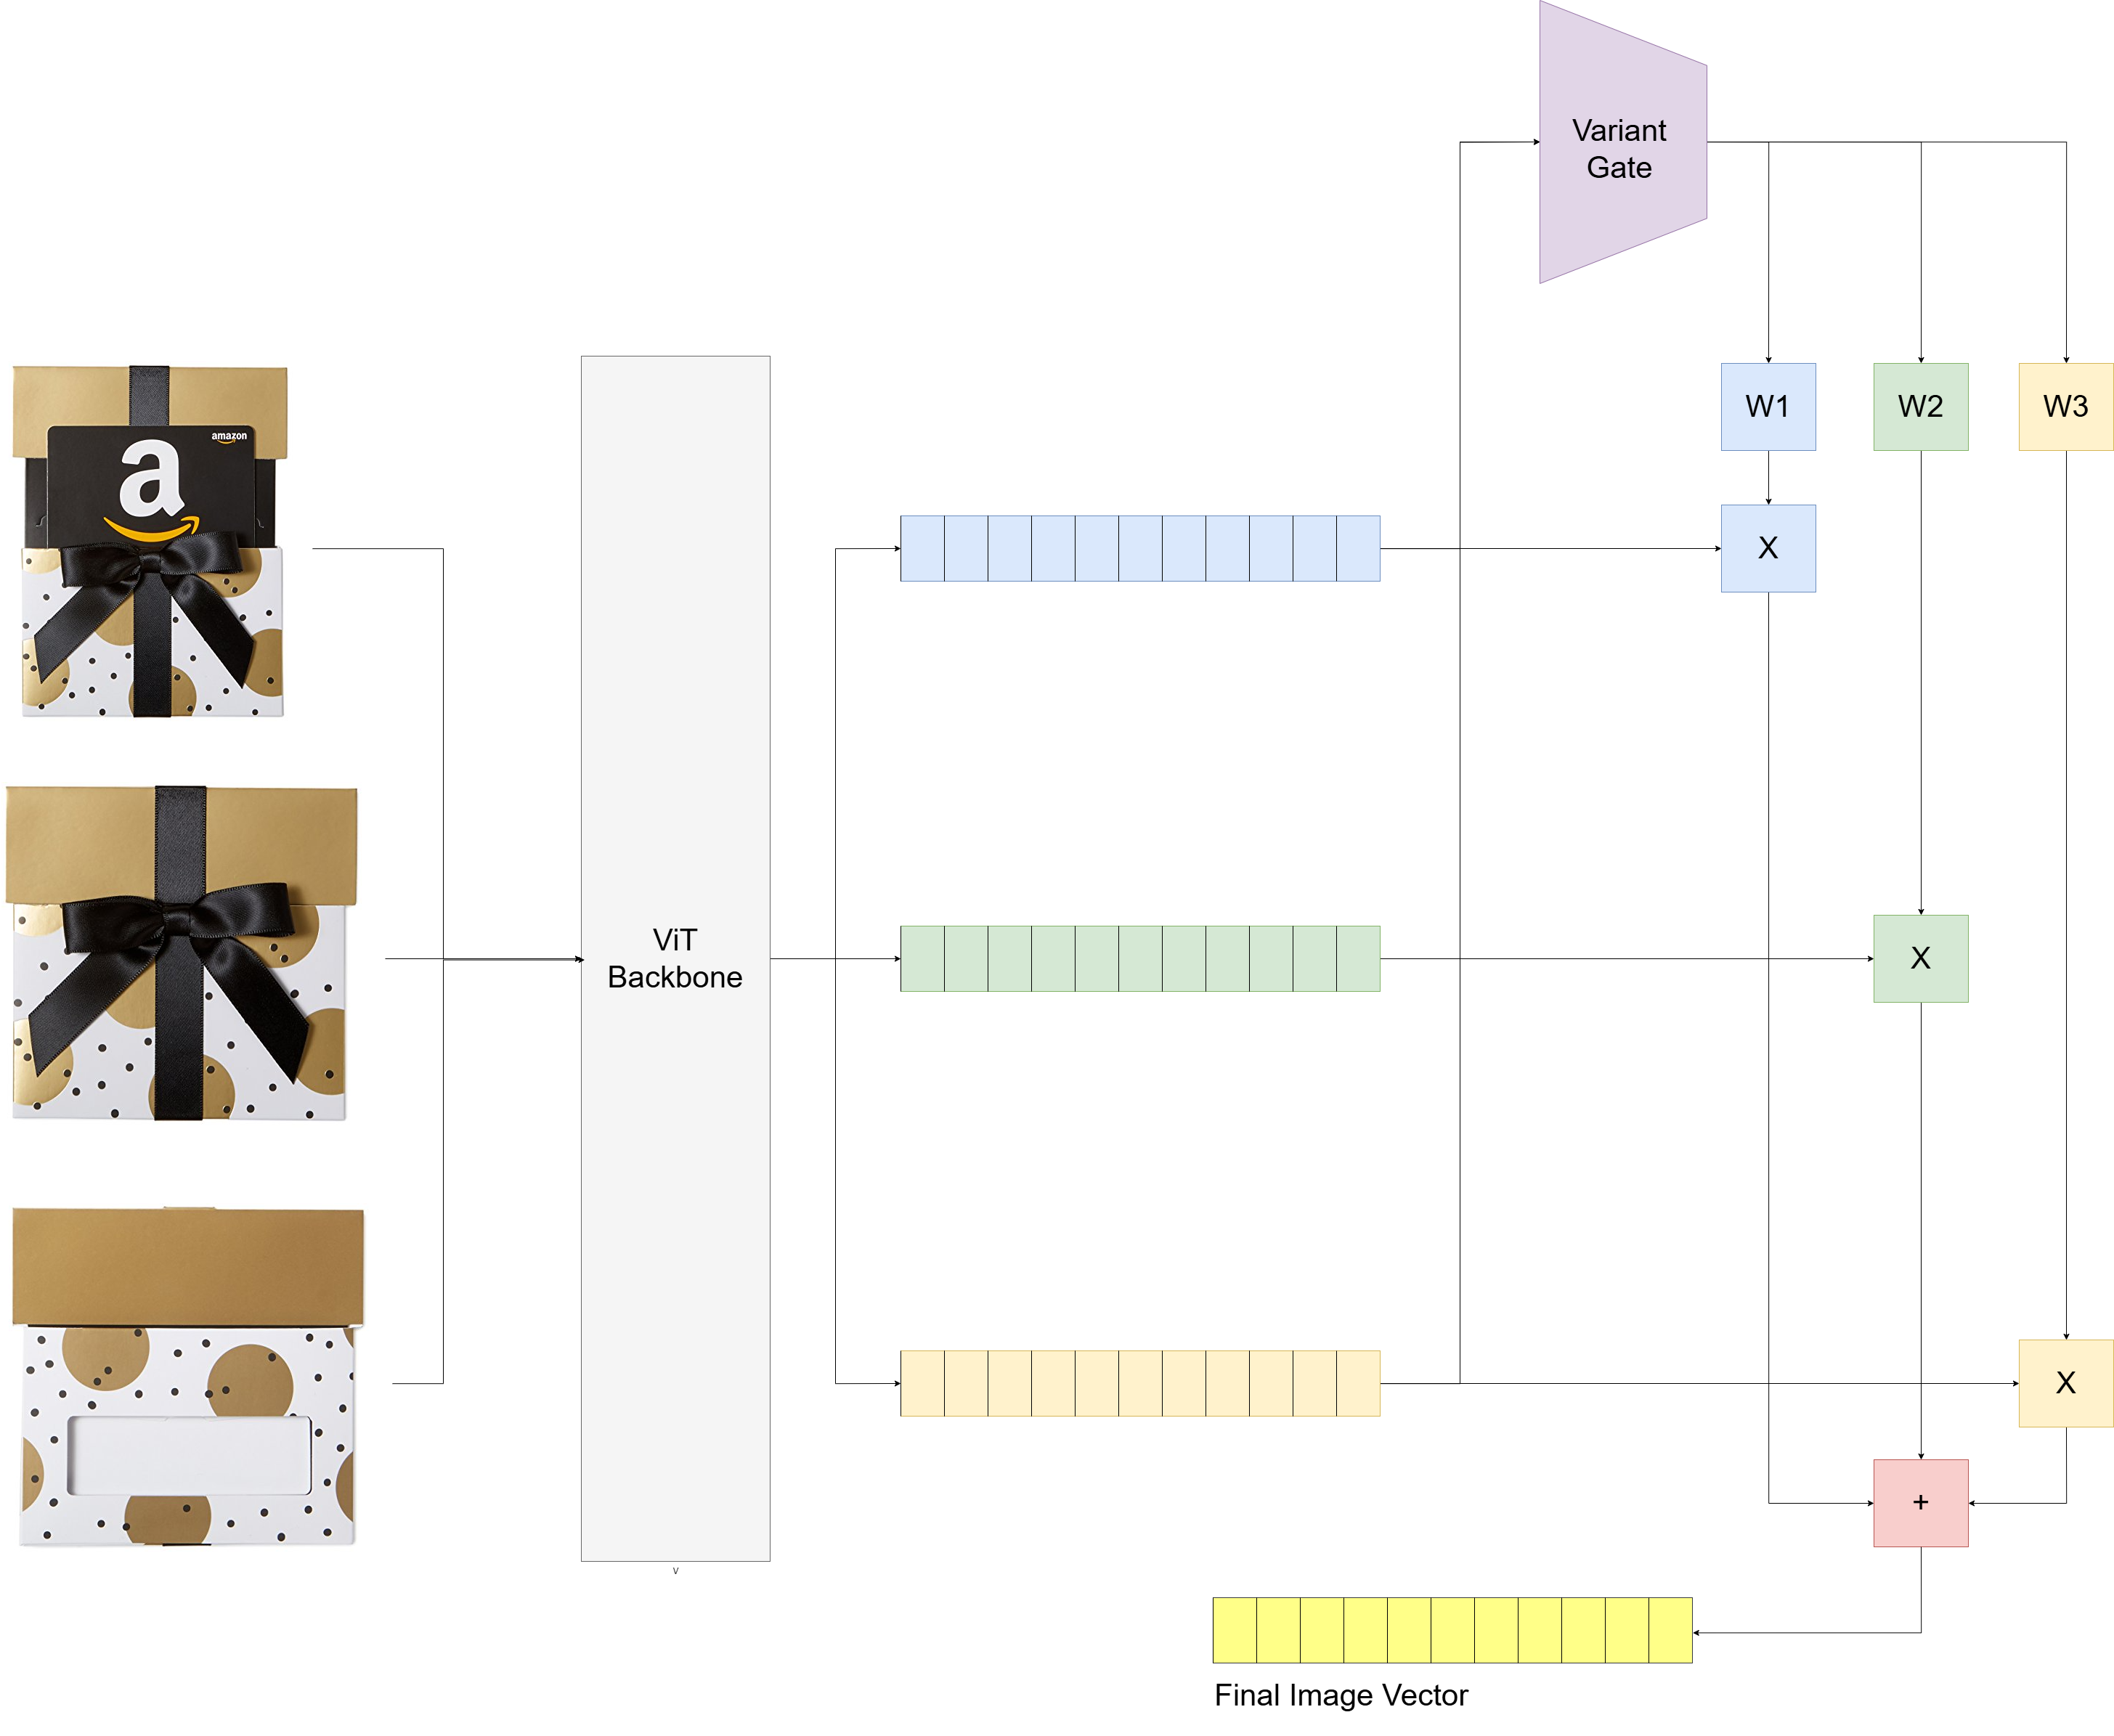
\includegraphics[width=0.8\textwidth]{Images/image_module.png} 
    \vspace{0.5cm}
    \caption{Quy trình Tính toán và Tổng hợp Đặc trưng Hình ảnh}
    \label{fig:image_module}
\end{figure}

Dựa trên sơ đồ kiến trúc tại Hình \ref{fig:image_module}, luồng xử lý hình ảnh được hiện thực hóa qua ba giai đoạn nối tiếp:

\begin{itemize}
    \item \textbf{Giai đoạn 1: Tiền xử lý (Preprocessing):} Nhằm đảm bảo tương thích với trọng số huấn luyện trước, mỗi hình ảnh được thay đổi kích thước về $224 \times 224$ pixels, chuyển đổi thành tensor \textit{Channel-first} trong khoảng $[0.0, 1.0]$, và cuối cùng được chuẩn hóa Z-score theo phân phối thống kê của tập ImageNet để đẩy nhanh tốc độ hội tụ.
    
    \item \textbf{Giai đoạn 2: Trích xuất đặc trưng và Chiếu không gian:} Các lô hình ảnh được đưa qua mô hình nền ViT tĩnh để sinh ra các vector đặc trưng thô. Ngay sau đó, một lớp tuyến tính (\texttt{self.proj}) thực hiện phép biến đổi không gian:
    \begin{equation}
        \mathbb{R}^{768} \rightarrow \mathbb{R}^{256}
    \end{equation}
    Phép nén này đồng bộ hóa hoàn toàn kích thước đặc trưng thị giác với tháp người dùng và luồng văn bản.
    
    \item \textbf{Giai đoạn 3: Tổng hợp đa ảnh và Chuẩn hóa:} Để xử lý bài toán không đồng nhất về số lượng biến thể ảnh, hệ thống áp dụng trực tiếp nguyên lý của Cơ chế Hợp nhất Không gian Vector đã được thiết lập lý thuyết tại Mục \ref{sec:attention_theory}. Luồng xử lý tại đây sử dụng một Cổng Biến thể đóng vai trò như mạng lưới sự chú ý để tự động học và phân bổ trọng số cho từng vector đặc trưng 256 chiều. Dựa trên bộ trọng số này, hệ thống thực hiện phép tính tổng có trọng số nhằm hội tụ các ảnh thành phần thành một vector đại diện duy nhất. Cơ chế này ép mô hình tự động điều hướng sự tập trung vào các bức ảnh sắc nét nhất mang tính đại diện cao và triệt tiêu tác động của ảnh nhiễu. Cuối cùng, hệ thống xử lý các vị trí khuyết dữ liệu đối với sản phẩm không có ảnh bằng cách điền ma trận không, đồng thời áp dụng chuẩn hóa L2 để xuất ra vector đặc trưng thị giác hoàn chỉnh, sẵn sàng cho khối hợp nhất đa phương thức phía sau.
    
\end{itemize}

\subsection{Tabular Encoder: Mô-đun Mã hóa Dữ liệu Bảng}

TabularEncoder chịu trách nhiệm mô hình hóa các thuộc tính siêu dữ liệu bao gồm điểm đánh giá và hệ thống phân loại. Mô-đun này được thiết kế theo luồng xử lý song song nhằm giải quyết hiệu quả bản chất hỗn hợp của dữ liệu bảng trước khi đồng bộ hóa không gian đặc trưng.

\vspace{0.3cm}
\noindent \textbf{1. Nhánh Xử lý Đặc trưng Phân loại}

Đối với các dữ liệu định danh rời rạc, hệ thống sử dụng các lớp mạng nhúng chuẩn \texttt{nn.Embedding} để ánh xạ chỉ số thành các vector đặc trưng không gian 32 chiều. Thiết kế bao gồm ba bảng nhúng độc lập phục vụ cho ba trường thông tin cốt lõi: Danh mục chính, Thương hiệu và Danh mục chi tiết. Riêng đối với trường Danh mục chi tiết mang đặc thù đa nhãn, một cơ chế tổng hợp nội bộ được áp dụng để tính toán ra một vector đại diện duy nhất cho toàn bộ tập hợp thẻ phân loại của sản phẩm.

\vspace{0.3cm}
\noindent \textbf{2. Nhánh Xử lý Đặc trưng Số thực}

Thay vì truyền trực tiếp dữ liệu thô vào lớp hợp nhất, hệ thống thiết lập một mạng nơ-ron đa tầng chuyên biệt để xử lý các thuộc tính định lượng như điểm đánh giá hay số lượt bình chọn hữu ích. Mạng nơ-ron này thực hiện chuỗi ba phép biến đổi liên tiếp: đầu tiên là phép chiếu mở rộng dữ liệu thô lên không gian ẩn 64 chiều, tiếp nối bằng hàm kích hoạt phi tuyến ReLU nhằm nắm bắt các tương quan không đơn điệu, và kết thúc bằng một lớp nén đưa dữ liệu về lại không gian mục tiêu 32 chiều. 

Sự thiết kế song song này đảm bảo toàn bộ đặc trưng định lượng và định danh đều được quy chuẩn về cùng một kích thước chiều, tạo điều kiện trơn tru nhất để nối ghép thành một vector dữ liệu bảng hoàn chỉnh, sẵn sàng tích hợp cùng đặc trưng văn bản và hình ảnh ở khối hợp nhất đa phương thức cuối cùng.

\vspace{0.3cm}
\noindent \textbf{3. Nhánh Hợp nhất Đặc trưng Bảng}

Tại tầng xử lý cuối cùng hay còn gọi là Lớp Hợp nhất, hệ thống thực hiện phép ghép nối chuỗi cho toàn bộ các vector đặc trưng phân loại và số thực đã qua tiền xử lý ở hai nhánh trên. Khối tensor tổng hợp này sau đó được truyền qua một mạng nơ-ron đa tầng để thực hiện ép kiểu và nén thông tin. Kết quả đầu ra là một vector đại diện duy nhất có kích thước không gian ẩn 256 chiều. Phép chiếu không gian ở giai đoạn cuối này đóng vai trò chốt chặn thiết yếu, đảm bảo đặc trưng siêu dữ liệu của sản phẩm được đồng bộ hoàn toàn về mặt kích thước với mô-đun văn bản và mô-đun hình ảnh, tạo tiền đề hoàn hảo cho giai đoạn dung hợp đa phương thức toàn cục.

\subsection{Cơ chế hợp nhất dữ liệu đa phương thức}

Đóng vai trò là thành phần chốt chặn cuối cùng trong kiến trúc Tháp Sản phẩm, cơ chế cổng hợp nhất chịu trách nhiệm tổng hợp các vector đặc trưng từ ba luồng dữ liệu riêng biệt: văn bản, hình ảnh và dữ liệu bảng. Dựa trên nền tảng lý thuyết về cơ chế chú ý đã được phân tích chi tiết tại \ref{sec:attention_theory}, đồ án tùy chỉnh module này để thực hiện phép hợp nhất có trọng số động. Cách tiếp cận này không chỉ giúp hệ thống tự động đánh giá mức độ đóng góp của từng phương thức dữ liệu đối với một mặt hàng cụ thể, mà còn cung cấp cơ chế xử lý linh hoạt cho thực trạng dữ liệu khuyết thiếu thường gặp trong môi trường thương mại điện tử.

\vspace{0.3cm}
\noindent \textbf{Tùy biến Mạng Gating dùng chung}

Thay vì sử dụng các mạng đánh giá độc lập, đồ án thiết kế một mạng Gating dùng chung cho toàn bộ các luồng dữ liệu nhằm đảm bảo sự công bằng và nhất quán trong thang đo. Kế thừa kiến trúc mạng truyền thẳng cơ sở, module này bao gồm một lớp tuyến tính nén phân nửa số chiều dữ liệu, kết hợp cùng hàm kích hoạt phi tuyến ReLU và một lớp đầu ra vô hướng. Điểm số vô hướng sinh ra đại diện cho mức độ tin cậy hay hàm lượng thông tin hữu ích mà mỗi nhánh dữ liệu mang lại cho bản sắc chung của sản phẩm.

\vspace{0.3cm}
\noindent \textbf{Quy trình tính toán và Xử lý khuyết thiếu}

Quy trình tính toán thực tế của đồ án được triển khai qua các bước tinh chỉnh chặt chẽ. Sau khi mạng Gating sinh ra các điểm số thô cho ba nhánh, hệ thống kích hoạt cơ chế xử lý ngoại lệ thông qua một ma trận mặt nạ. Ma trận này làm nhiệm vụ quét và phát hiện các luồng thông tin không tồn tại, chẳng hạn như sản phẩm thiếu ảnh minh họa, từ đó gán ngay một giá trị âm vô cùng xấp xỉ $-10^9$ cho điểm số tương ứng. Bước can thiệp kỹ thuật này đóng vai trò sống còn trước khi đưa dữ liệu qua hàm Softmax, đảm bảo trọng số phân bổ cho các thành phần bị khuyết sẽ tự động triệt tiêu về $0$, qua đó cách ly hoàn toàn xung nhiễu khỏi vector tổng hợp.

Sau bước lọc nhiễu, hệ thống áp dụng hàm Softmax để chuyển hóa các điểm số thô thành một phân phối xác suất có tổng bằng $1$. Trọng số động của luồng văn bản, hình ảnh và dữ liệu bảng lần lượt được xác định qua ma trận:
\begin{equation}
    \mathbf{W} = \text{Softmax}(\mathbf{G}) = [w_t, w_i, w_b]
\end{equation}

Vector hợp nhất cuối cùng $\mathbf{v}_{\text{fused}}$ được đồ án thiết lập dựa trên phép cộng có trọng số của các vector thành phần:
\begin{equation}
    \mathbf{v}_{\text{fused}} = w_t \cdot \mathbf{e}_{\text{text}} + w_i \cdot \mathbf{e}_{\text{img}} + w_b \cdot \mathbf{e}_{\text{tab}}
\end{equation}

Để hoàn thiện, kết quả này trải qua phép chuẩn hóa L2 nhằm đưa vector về độ dài đơn vị. Bước chuẩn hóa này tạo ra vector đại diện sản phẩm hoàn chỉnh, đảm bảo tính ổn định và tính đẳng hướng tối đa khi tham gia vào các phép tính toán độ tương đồng Cosine trong không gian truy xuất toàn cục phía sau.

\section{Xây dựng Tháp Người dùng}

\subsection{Tổng quan và Nền tảng Kỹ thuật}
Tháp người dùng đảm nhận vai trò mô hình hóa sở thích và hành vi của người dùng dựa trên lịch sử tương tác. Khác biệt với các phương pháp lọc cộng tác truyền thống vốn coi sở thích là yếu tố tĩnh, module này tiếp cận bài toán dưới góc độ Gợi ý Tuần tự (\textit{Sequential Recommendation}). Mục tiêu cốt lõi là học được một vector biểu diễn người dùng $\mathbf{u}_t$ tại thời điểm $t$, sao cho vector này bao hàm được ý định mua sắm tiếp theo dựa trên chuỗi $n$ tương tác quá khứ $S = \{i_1, i_2, \dots, i_t\}$, trong đó $i_k$ là sản phẩm mà người dùng đã tương tác tại bước thứ $k$.

Về mặt nền tảng kỹ thuật, hệ thống sử dụng kiến trúc Transformer Encoder lấy cảm hứng từ mô hình SASRec \cite{7}. Việc lựa chọn kiến trúc này cho phép mô hình vượt qua hạn chế của các mạng RNN hay CNN truyền thống trong việc nắm bắt các mối quan hệ phụ thuộc dài hạn, từ đó hiểu sâu hơn về sự chuyển dịch trong thị hiếu người dùng theo thời gian.

\subsection{Cơ chế Biểu diễn Người dùng}
Để kiến tạo không gian biểu diễn người dùng phong phú, hệ thống xử lý chuỗi dữ liệu đầu vào thu được từ giai đoạn tiền xử lý. Mỗi phần tử trong chuỗi này là một tổ hợp thông tin bao gồm nội dung nhận xét của người dùng về sản phẩm và vector đặc trưng $\mathbf{v}_{\text{item}}$ của chính sản phẩm đó. Để đồng bộ hóa dữ liệu văn bản phi cấu trúc vào không gian tính toán chung, nhóm thực hiện biến đổi các nhận xét thông qua bộ mã hóa chuyên biệt dưới đây.

\subsubsection{ReviewTextEncoder và Chiến lược Chia sẻ Trọng số}
Trong kiến trúc Tháp Người dùng, thành phần mã hóa văn bản chịu trách nhiệm chuyển đổi nội dung bình luận tổng hợp thành các vector đặc trưng ngữ nghĩa. Một đặc điểm kiến trúc quan trọng trong thiết kế của hệ thống là việc áp dụng cơ chế Chia sẻ Trọng số (\textit{Weight Sharing}). Cụ thể, bộ mã hóa văn bản trong Tháp Người dùng không được khởi tạo độc lập mà sử dụng chung kiến trúc mạng và toàn bộ bộ tham số đã được huấn luyện của bộ mã hóa trong Tháp Sản phẩm. Điều này đồng nghĩa với việc các văn bản đánh giá của người dùng và mô tả sản phẩm đều được xử lý qua cùng một mô hình ngôn ngữ tiền huấn luyện và cùng một lớp chiếu không gian.

Chiến lược chia sẻ trọng số này mang lại ba lợi ích kỹ thuật thiết yếu. Thứ nhất, nó đảm bảo sự đồng bộ tuyệt đối về không gian ngữ nghĩa, giúp các văn bản từ phía người dùng và sản phẩm được ánh xạ vào cùng một hệ quy chiếu vector, tạo điều kiện thuận lợi cho mô hình trong việc so sánh và tìm kiếm sự tương đồng giữa lời nhận xét và mô tả sản phẩm. Thứ hai, cơ chế này giúp tối ưu hóa tài nguyên tính toán bằng cách giảm đáng kể số lượng tham số cần lưu trữ, tránh việc hệ thống phải duy trì hai mô hình ngôn ngữ lớn riêng biệt. Cuối cùng, Tháp Người dùng có thể thừa hưởng trực tiếp khả năng hiểu ngôn ngữ đã được tinh chỉnh từ quá trình huấn luyện Tháp Sản phẩm, giúp quá trình hội tụ diễn ra nhanh hơn.

Về mặt cài đặt kỹ thuật, module này tiếp nhận đầu vào là danh sách các chuỗi văn bản đánh giá trong lịch sử hành vi và trả về một tensor có kích thước $[B, S, D_{\text{latent}}]$, tương ứng với kích thước lô, độ dài chuỗi lịch sử và kích thước vector đặc trưng $256$ chiều.

\subsubsection{ReviewTabularEncoder: Mô-đun Mã hóa Cấu trúc Đánh giá}
Mô-đun \texttt{ReviewTabularEncoder} chịu trách nhiệm mã hóa các thông tin định lượng và định danh gắn liền với bài đánh giá, bao gồm ba trường dữ liệu cốt lõi: điểm đánh giá (\textit{Rating}) trong thang đo $1-5$, số lượt bình chọn hữu ích (\textit{Helpful Votes}) và trạng thái xác thực mua hàng (\textit{Verified Purchase}). Mục tiêu của mô-đun là chuyển đổi các tín hiệu thô này thành một vector đặc trưng thống nhất, bổ sung ngữ cảnh tin cậy cho nội dung văn bản.

\vspace{0.3cm}
\noindent \textbf{Kiến trúc Mạng và Các Khối Xử lý}

Hệ thống được thiết kế với ba khối xử lý chuyên biệt tương ứng với đặc thù của từng loại dữ liệu. Đối với thuộc tính phân loại như trạng thái xác thực mua hàng, hệ thống sử dụng lớp \texttt{nn.Embedding} để chuyển đổi dữ liệu rời rạc sang không gian vector liên tục. Không gian nhúng được thiết lập với 3 trạng thái bao gồm giá trị đệm, đã mua và chưa xác thực, được ánh xạ vào vector có kích thước mặc định là $4$ chiều.

Đối với dữ liệu số học, một mạng Perceptron đa lớp (MLP) được thiết kế để biến đổi cặp giá trị điểm số và lượt bình chọn từ không gian 2 chiều sang không gian đặc trưng cao chiều hơn. Kiến trúc mạng bao gồm lớp ẩn $64$ chiều kết hợp với hàm kích hoạt ReLU, sau đó nén xuống $32$ chiều. Thiết kế này cho phép mô hình nắm bắt các tương tác phi tuyến tính phức tạp giữa điểm số và mức độ tin cậy của cộng đồng, ví dụ như sự khác biệt ngữ nghĩa giữa một đánh giá điểm thấp nhưng nhận được nhiều sự đồng tình so với một đánh giá điểm thấp nhưng ít được quan tâm.

Tại tầng xử lý cuối cùng, Khối Hợp nhất (\textit{Fusion Block}) chịu trách nhiệm tổng hợp thông tin từ nhánh số học $32$ chiều và nhánh phân loại $4$ chiều. Vector ghép nối có kích thước tổng thể là $36$ được đưa qua một mạng nơ-ron đa lớp để tạo ra đầu ra cuối cùng. Điểm đáng lưu ý trong thiết kế là lớp cuối cùng được cấu hình là lớp tuyến tính thuần túy không kèm hàm kích hoạt. Thiết kế này cho phép vector đầu ra nhận các giá trị thực trong toàn miền $(-\infty, +\infty)$, giúp bảo toàn sự phong phú của thông tin (\textit{information richness}) trước khi được tích hợp vào các lớp tiếp theo của Tháp Người dùng.

\vspace{0.3cm}
\noindent \textbf{Quy trình Xử lý Luồng Dữ liệu}

Quy trình xử lý diễn ra theo trình tự chặt chẽ nhằm đảm bảo tính toàn vẹn của dữ liệu. Đầu vào bao gồm điểm số, lượt bình chọn và trạng thái xác thực sau khi được làm sạch và chuẩn hóa sẽ được phân tách vào các nhánh xử lý tương ứng. Trạng thái xác thực đi qua lớp Embedding để tạo vector $\mathbf{v}_{\text{cat}}$, trong khi điểm số và lượt bình chọn đi qua mạng chiếu số học để tạo vector $\mathbf{v}_{\text{num}}$. Hai thành phần này sau đó được ghép nối thành vector tổng hợp $\mathbf{v}_{\text{concat}}$ theo công thức:
\begin{equation}
    \mathbf{v}_{\text{concat}} = [\mathbf{v}_{\text{num}}; \mathbf{v}_{\text{cat}}]
\end{equation}
Cuối cùng, vector tổng hợp được đưa qua mạng Fusion để tạo ra biểu diễn vector đầu ra, đại diện cho ngữ cảnh cấu trúc toàn diện của bài đánh giá.

\subsubsection{Cổng Hợp nhất Người dùng (User Fusion Gate)}

Cổng \texttt{GatingFusionLayer} đóng vai trò trung tâm trong việc tổng hợp vector biểu diễn tương tác của người dùng. Nhiệm vụ cốt lõi của thành phần này là kết hợp vector định danh sản phẩm $\mathbf{v}_{\text{item}}$ thu được từ Tháp Sản phẩm với ngữ cảnh tương tác cụ thể, bao gồm nội dung đánh giá $\mathbf{v}_{\text{text}}$ và các chỉ số định lượng $\mathbf{v}_{\text{tabular}}$. Mục tiêu là tạo ra một vector duy nhất $\mathbf{h}_{\text{seq}}$ đại diện cho một bước trong chuỗi hành vi thông qua cơ chế \textit{Gating}, cho phép mô hình tự động điều chỉnh mức độ đóng góp của từng nguồn thông tin dựa trên ngữ cảnh thực tế.

\vspace{0.3cm}
\noindent \textbf{Kiến trúc và Các Khối Xử lý}

Về mặt kiến trúc, module bao gồm hai khối xử lý song song. Khối Chiếu và Đồng bộ sử dụng ba lớp tuyến tính riêng biệt để đưa các vector đầu vào có kích thước khác nhau về cùng một không gian chiều chung $d_{\text{model}} = 256$, chuẩn bị cho quá trình cộng gộp. Song song đó, Mạng \textit{Gating} được thiết kế dưới dạng một mạng perceptron đa lớp ($\text{Linear} \to \text{ReLU} \to \text{Linear}$) tiếp nhận toàn bộ dữ liệu ghép nối đầu vào để tính toán điểm số tầm quan trọng cho từng thành phần Item, Text và Tabular.

\vspace{0.3cm}
\noindent \textbf{Quy trình Xử lý}

Quy trình xử lý diễn ra tuần tự qua ba bước. Đầu tiên, các vector đặc trưng được chiếu sang không gian chung và áp dụng hàm kích hoạt phi tuyến ReLU để tăng khả năng biểu diễn. Kế đến, hệ thống thực hiện tính toán trọng số thông qua hàm Softmax, tái sử dụng cơ chế hợp nhất động tương tự như đã trình bày tại phần Tháp Sản phẩm, nhưng áp dụng cho ngữ nghĩa kết hợp giữa sản phẩm và phản hồi người dùng. Kết quả đầu ra là một tensor có kích thước $[B, S, D_{\text{latent}}]$, sẵn sàng làm đầu vào cho mạng \textit{Transformer Encoder} để mô hình hóa chuỗi thời gian.

\subsubsection{Module Mã hóa Vị trí (Positional Encoding)}

Trong kiến trúc Tháp Người dùng, chuỗi hành vi lịch sử được xử lý thông qua mạng Transformer. Một đặc điểm cố hữu của cơ chế \textit{Self-Attention} là tính bất biến hoán vị, nghĩa là mô hình xử lý tập hợp đầu vào song song mà không tự nhận biết được thứ tự trước sau của các phần tử. Tuy nhiên, đối với bài toán gợi ý tuần tự, thứ tự tương tác đóng vai trò tối quan trọng, chẳng hạn như hành vi mua điện thoại thường mang tính tiền đề và diễn ra trước khi mua ốp lưng. Để khắc phục hạn chế này, module \texttt{PositionalEncoding} được thiết kế nhằm bổ sung thông tin về vị trí tương đối hoặc tuyệt đối vào các vector biểu diễn trước khi chúng được đưa vào các lớp Attention.

\vspace{0.3cm}
\noindent \textbf{Phương pháp Mã hóa Sinusoidal}

Hệ thống áp dụng phương pháp Mã hóa Sinusoidal cố định theo kiến trúc Transformer nguyên bản. Phương pháp này tận dụng các hàm lượng giác với tần số biến thiên để tạo ra một đặc trưng vị trí độc nhất cho mỗi bước thời gian.

% \begin{figure}[H]
%     \centering
%     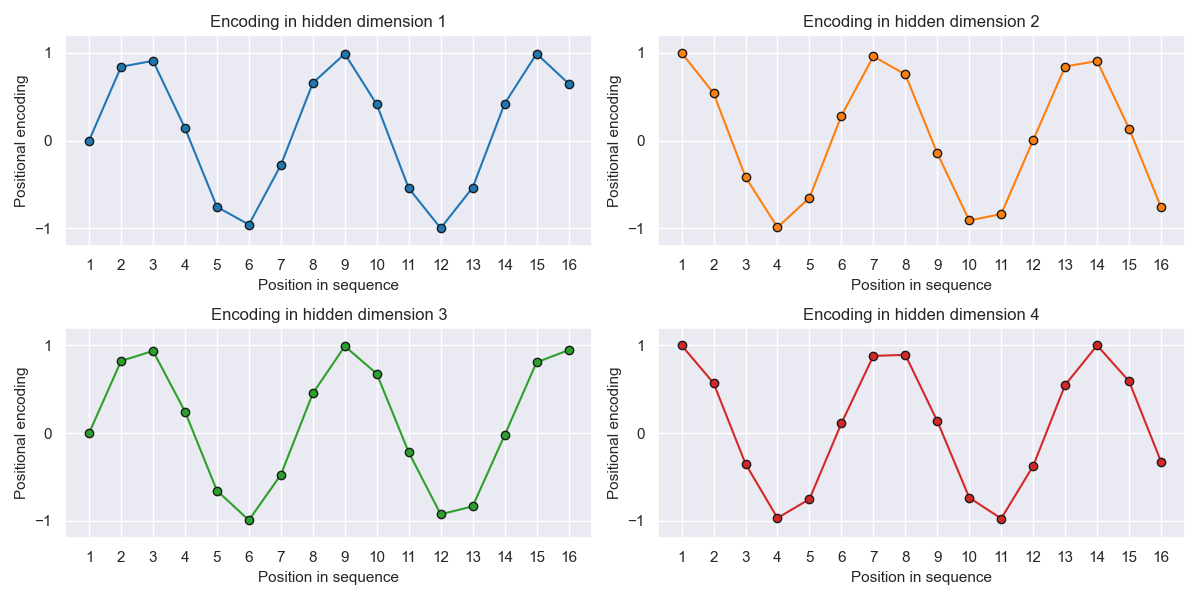
\includegraphics[width=1.0\textwidth]{Images/position_encoder.png}
%     \vspace{0.3cm}
%     \caption{Minh họa trực quan giá trị Positional Encoding trên 4 chiều ẩn đầu tiên. Các đường cong hình sin với tần số khác nhau giúp mô hình phân biệt vị trí trong chuỗi.}
%     \label{fig:pos_encoding_vis}
% \end{figure}


Dựa trên đề xuất của Vaswani và cộng sự \cite{12}, giá trị mã hóa tại vị trí $pos$ và chiều $i$ trong không gian vector kích thước $d_{\text{model}}$ được xác định bởi công thức toán học sau:
\begin{align}
    \text{PE}_{(pos, 2i)} &= \sin\left(\frac{pos}{10000^{2i/d_{\text{model}}}}\right) \\
    \text{PE}_{(pos, 2i+1)} &= \cos\left(\frac{pos}{10000^{2i/d_{\text{model}}}}\right)
\end{align}
Trong đó, các chiều chẵn $2i$ được áp dụng hàm Sine và các chiều lẻ $2i+1$ được áp dụng hàm Cosine. Việc kết hợp hai hàm lượng giác này cho phép mô hình lan truyền và ngoại suy thông tin vị trí một cách hiệu quả ngay cả đối với các chuỗi dài hơn độ dài đã gặp trong quá trình huấn luyện.

\noindent \textbf{Chi tiết Kỹ thuật và Quy trình Cài đặt}

Mô-đun được hiện thực hóa dưới dạng một lớp kế thừa từ \texttt{nn.Module} với quy trình xử lý được tối ưu hóa ngay từ bước khởi tạo. Cụ thể, một ma trận vị trí \texttt{pe} có kích thước $[\texttt{max\_len}, 1, d_{\text{model}}]$ được tính toán trước và lưu trữ vào bộ nhớ đệm thông qua cơ chế \texttt{register\_buffer}. Kỹ thuật này cho phép hệ thống ghi nhận ma trận như một phần trạng thái bền vững của mô hình nhưng không tham gia vào quá trình cập nhật gradient, giúp cố định thông tin vị trí và giảm tải số lượng tham số cần tối ưu.

Trong quá trình lan truyền xuôi, các vector vị trí tương ứng được cộng trực tiếp vào vector đặc trưng đầu vào theo công thức:
\begin{equation}
    \mathbf{x} = \mathbf{x} + \mathbf{PE}[:\texttt{x.size(0)}]
\end{equation}
Phép toán cộng tuyến tính này đóng vai trò quyết định giúp cơ chế \textit{Attention} phân biệt được các thực thể giống nhau nhưng xuất hiện tại các thời điểm khác nhau trong chuỗi hành vi, đảm bảo tính thứ tự của dữ liệu. Nhằm tăng cường khả năng tổng quát hóa, một lớp \texttt{Dropout} với tỷ lệ mặc định $0.1$ được áp dụng ngay sau bước cộng mã hóa. Thao tác này giúp ngăn chặn hiện tượng quá khớp bằng cách buộc mô hình học các mẫu cấu trúc tổng quát thay vì phụ thuộc thái quá vào thông tin vị trí tuyệt đối.

Trong ngữ cảnh cụ thể của hệ thống gợi ý, thành phần này nắm giữ vai trò then chốt trong việc mô hình hóa tính gần đây và nguyên tắc nhân quả. Nó cung cấp cơ sở tham chiếu để mô hình nhận thức được khoảng cách thời gian giữa các tương tác, từ đó tạo điều kiện cho cơ chế \textit{Self-Attention} phân bổ trọng số hợp lý: ưu tiên cao hơn cho các hành vi gần đây đại diện cho sở thích ngắn hạn, đồng thời vẫn duy trì ngữ cảnh dài hạn để đảm bảo độ chính xác trong việc dự báo hành động tiếp theo.

\subsubsection{Cơ chế Tạo và Tổng hợp Vector Người dùng}

Nhiệm vụ cốt lõi của phân hệ này là thực hiện chuyển đổi chuỗi các trạng thái ẩn tuần tự — vốn là đầu ra từ mạng \textit{Transformer} — thành một vector duy nhất đại diện cho chân dung sở thích toàn diện của người dùng. Quy trình này được xây dựng dựa trên sự kết hợp chặt chẽ giữa kỹ thuật mô hình hóa chuỗi thời gian và các phương pháp tổng hợp thông tin có chọn lọc.

\noindent \textbf{Quy trình Xử lý và Tổng hợp Vector Người dùng}

\begin{figure}[H]
    \centering
    
\includegraphics[width=0.95\linewidth]{images/user_tower.png} 
    \vspace{0.5cm}
    \caption{Kiến trúc chi tiết Tháp Người dùng với cơ chế mô hình hóa chuỗi đa phương thức.}
    \label{fig:user_tower_arch}
\end{figure}

Sơ đồ minh họa luồng xử lý dữ liệu tuần tự bên trong Tháp Người dùng, được thiết kế để chuyển đổi lịch sử hành vi phức tạp thành một vector đại diện sở thích duy nhất. Quá trình này diễn ra qua bốn giai đoạn xử lý phân tầng từ dưới lên trên:

\begin{itemize}
    \item \textbf{1. Tầng Mã hóa Đặc trưng Chia sẻ (\textit{Shared Encoders Layer}):} \\
    Tại mỗi bước thời gian trong chuỗi hành vi, hệ thống tiếp nhận bộ ba dữ liệu đầu vào gồm nội dung văn bản đánh giá, thông tin bảng số liệu và định danh sản phẩm. Các luồng dữ liệu này được đưa qua khối các bộ mã hóa chuyên biệt (\textit{Encoders}). Điểm đặc biệt trong thiết kế này là cơ chế chia sẻ trọng số (\textit{Share weight}), nghĩa là cùng một bộ tham số mã hóa được sử dụng lặp lại cho mọi bước thời gian và đồng bộ hoàn toàn với các bộ mã hóa tại Tháp Sản phẩm. Điều này đảm bảo tính nhất quán về không gian đặc trưng giữa hai tháp mô hình.

    \item \textbf{2. Tầng Hợp nhất Cục bộ (\textit{Fusion Gate}):} \\
    Sau khi trích xuất đặc trưng sơ cấp, tại mỗi bước thời gian, các vector thành phần được đưa qua cổng hợp nhất \textit{Fusion Gate}. Module này chịu trách nhiệm tổng hợp ba nguồn thông tin không đồng nhất thành một vector đại diện duy nhất (\textit{Vector Review}), gói gọn toàn bộ ngữ cảnh tương tác của người dùng tại thời điểm đó.

    \item \textbf{3. Tầng Mô hình hóa Tuần tự (\textit{Sequence Modeling Layer}):} \\
    Để mô hình nhận thức được thứ tự của các hành vi, giải thuật Mã hóa Vị trí (\textit{Positional Encoding}) được cộng trực tiếp vào các vector đặc trưng. Chuỗi vector sau khi đã tích hợp thông tin vị trí được đưa vào khối \textit{Transformer Encoder Block}. Tại đây, cơ chế \textit{Self-Attention} cho phép mô hình học các mối quan hệ phụ thuộc dài hạn và nắm bắt sự chuyển dịch trong thị hiếu người dùng qua thời gian.
\end{itemize}

Giai đoạn tiếp theo tập trung vào việc Tổng hợp Đặc trưng. Do độ dài lịch sử hành vi của người dùng mang tính biến thiên, hệ thống áp dụng kỹ thuật \textit{Masked Mean Pooling} để nén toàn bộ chuỗi trạng thái ẩn từ Transformer thành một vector đại diện duy nhất. Để thực hiện điều này, mặt nạ đệm ban đầu được xử lý và mở rộng chiều tương thích với tensor dữ liệu, trong đó các vị trí chứa thông tin thực được gán trọng số $1$ và vị trí đệm nhận giá trị $0$. Hệ thống tiến hành nhân từng phần tử giữa đầu ra mô hình và mặt nạ trọng số nhằm triệt tiêu hoàn toàn các vector tại vị trí đệm về vector $\mathbf{0}$, sau đó cộng dồn các đặc trưng dọc theo trục thời gian. Vector đại diện cuối cùng được xác định bằng cách chia tổng thu được cho số lượng hành vi thực tế, với việc bổ sung một hằng số nhỏ $\epsilon$ vào mẫu số để đảm bảo tính ổn định số học:
\begin{equation}
    \mathbf{u}_{\text{pooled}} = \frac{\sum_{t=1}^{T} (\mathbf{h}_t \cdot m_t)}{\sum_{t=1}^{T} m_t + \epsilon}
\end{equation}
Trong đó $\mathbf{h}_t$ là trạng thái ẩn tại bước $t$ và $m_t$ là giá trị mặt nạ nhị phân.

\vspace{0.2cm}

Quy trình khép lại bằng giai đoạn Tinh chỉnh và Chuẩn hóa. Vector trung bình sau khi tính toán được đưa qua một lớp Tuyến tính cuối cùng đóng vai trò như bộ chuyển đổi đặc trưng cao cấp, tối ưu hóa cho việc so khớp với sản phẩm. Đầu ra cuối cùng trải qua phép chuẩn hóa L2 để đưa về độ dài đơn vị trên mặt cầu, đảm bảo khoảng cách giữa người dùng và sản phẩm được đo lường chính xác và nhất quán thông qua độ tương đồng Cosine.

\section{Chiến lược Huấn luyện Hai giai đoạn}

Việc tối ưu hóa đồng thời các hàm mất mát tương phản nội bộ tháp sản phẩm và toàn cục giữa hai tháp trong một đồ thị tính toán duy nhất thường dẫn đến hiện tượng xung đột đạo hàm, đồng thời tiêu tốn lượng lớn tài nguyên bộ nhớ VRAM. Để khắc phục thách thức này và đảm bảo mô hình hội tụ ổn định, đồ án đề xuất áp dụng chiến lược huấn luyện hai giai đoạn. Quá trình này tách biệt việc thấu hiểu nội dung sản phẩm và việc nắm bắt hành vi người dùng thành hai bước tuần tự

\subsection{Giai đoạn 1: Tiền huấn luyện độc lập Tháp Sản phẩm}

Trong giai đoạn đầu tiên, để ngăn chặn tín hiệu nhiễu từ chuỗi lịch sử tương tác, cấu trúc Tháp Người dùng bị loại bỏ hoàn toàn khỏi đồ thị tính toán. Hệ thống chỉ tập trung cấp phát tài nguyên phần cứng để tối ưu hóa mạng nơ-ron của Tháp Sản phẩm. Đồ án sử dụng kho dữ liệu sản phẩm tĩnh bao gồm hình ảnh, văn bản mô tả và các thuộc tính dạng bảng làm tập dữ liệu huấn luyện.

Thành phần cốt lõi trong chiến lược tối ưu hóa của hệ thống là hàm mất mát dựa trên nguyên lý Học tương phản. Cụ thể, đồ án áp dụng biến thể \textit{Symmetric InfoNCE Loss}, phương pháp đã chứng minh hiệu quả vượt trội qua sự thành công của mô hình CLIP \cite{13}. Khác với các hàm mất mát truyền thống, phương pháp này thực hiện tính toán độ tương đồng chéo giữa các cặp dữ liệu đa phương thức theo cả hai chiều nhằm đồng bộ hóa không gian biểu diễn chung. Mục tiêu tối thượng là tối ưu hóa không gian vector sao cho các cặp dữ liệu tương ứng như hình ảnh và văn bản của cùng một sản phẩm sẽ có vector biểu diễn gần nhau do lực hút, trong khi các cặp dữ liệu không tương ứng bị đẩy ra xa nhau do lực đẩy.

Mặc dù hàm mất mát \textit{InfoNCE} thể hiện sự ưu việt trong việc đồng bộ hóa không gian biểu diễn toàn cục, nó vẫn bộc lộ hạn chế khi xử lý các tập dữ liệu có độ hạt mịn (fine-grained) và độ tương đồng nội nhóm cao, điển hình như miền dữ liệu Amazon Beauty. Trong không gian này, các mặt hàng thường có sự chồng chéo lớn về đặc trưng (ví dụ: các sản phẩm mỹ phẩm cùng chủng loại nhưng khác thương hiệu). Hàm \textit{InfoNCE} có xu hướng phân bổ lực đẩy đồng đều lên mọi mẫu âm tính trong lô, dẫn đến việc thiếu sự tập trung cần thiết để phân tách các sản phẩm cực kỳ giống nhau.

Để khắc phục hạn chế của hàm mất mát InfoNCE khi xử lý các tập dữ liệu có độ tương đồng nội nhóm cao, đồ án tích hợp thêm hàm Batch-Hard Triplet Loss vào giai đoạn tinh chỉnh. Thay vì dàn trải lực tối ưu đồng đều, phương pháp này chỉ tập trung xử lý mẫu đối nghịch khó nhất, tức là sản phẩm nhiễu có vị trí gần với mục tiêu nhất trong không gian vector. Dựa trên ma trận tương đồng Cosine giữa hai tập hợp biểu diễn, mô hình thiết lập một ranh giới an toàn $m$ nhằm ép buộc độ tương đồng của cặp dữ liệu mục tiêu phải luôn vượt trội hơn mẫu âm tính khó nhất một khoảng tối thiểu bằng $m$. Quá trình này được tính toán đối xứng theo cả hai chiều để đảm bảo tính đồng nhất của kiến trúc Hai tháp. Sự kết hợp giữa khả năng quy hoạch không gian toàn cục của InfoNCE và khả năng tinh chỉnh chi tiết cục bộ của Batch-Hard Triplet Loss giúp hệ thống xây dựng một không gian nhúng mạnh mẽ, qua đó phân biệt chính xác các mặt hàng có đặc điểm cực kỳ giống nhau trong những miền dữ liệu phức tạp.

\noindent \textbf{Vai trò chiến lược trong hệ thống gợi ý}

Trong kiến trúc đa phương thức của đề tài, hàm mất mát tương phản đóng vai trò then chốt trong việc định hình không gian biểu diễn. Chức năng quan trọng nhất của nó là đồng bộ hóa không gian vector, hoạt động như một lực hấp dẫn để kéo các biểu diễn đặc trưng từ các nguồn dữ liệu phân tán như văn bản, hình ảnh và dữ liệu bảng về cùng một không gian ngữ nghĩa thống nhất. Bên cạnh đó, thông qua việc phân biệt rõ ràng giữa các cặp tương ứng và không tương ứng trong lô dữ liệu, mô hình học được khả năng trích xuất các đặc trưng độc đáo mang tính phân biệt cao. Đây là tiền đề quan trọng giúp tối ưu hóa khả năng truy xuất ứng viên, nâng cao độ chính xác trong việc tìm kiếm và gợi ý sản phẩm phù hợp.

\subsection{Giai đoạn 2: Tinh chỉnh toàn cục đa tháp}

\noindent \textbf{Cơ chế Mẫu âm tính kết hợp}

Hàm mất mát toàn cục được thiết kế dựa trên sự kết hợp giữa chiến lược lấy mẫu âm tính trong lô và cơ chế tiêm mẫu âm tính rõ ràng. Thông thường, hệ thống chỉ tận dụng các sản phẩm khác trong cùng một lô huấn luyện làm mẫu đối nghịch giả định, với rủi ro rằng người dùng có thể vẫn thích chúng nhưng chưa có cơ hội tương tác. Để tối ưu hóa không gian biểu diễn và tận dụng tối đa phản hồi thực tế, đồ án bổ sung thêm cho mỗi người dùng một vector đại diện cho sản phẩm mà họ đã trực tiếp đánh giá thấp.

Giả sử một lô huấn luyện có kích thước $N=3$. Khi xem xét người dùng thứ nhất $u_1$, sản phẩm $v_1^+$ ở cùng chỉ số index được coi là cặp dương tính. Các sản phẩm $v_2^+$ và $v_3^+$ tự động trở thành mẫu âm tính trong lô. Đặc biệt, một sản phẩm $v_1^-$ do chính $u_1$ đánh giá thấp được ghép thêm vào không gian đối nghịch, tạo ra một rào cản ngữ nghĩa mạnh mẽ. Cơ chế này được minh họa chi tiết tại Bảng \ref{tab:in_batch_negatives}.

\begin{table}[H]
    \centering
    \caption{Minh họa cơ chế lấy mẫu kết hợp với kích thước lô $N=3$}
    \label{tab:in_batch_negatives}
    \renewcommand{\arraystretch}{1.5}
    \footnotesize
    \begin{tabularx}{\textwidth}{|>{\centering\arraybackslash}m{2.5cm}|>{\centering\arraybackslash}X|>{\centering\arraybackslash}X|>{\centering\arraybackslash}X|>{\centering\arraybackslash}X|}
    \hline
    \textbf{Người dùng \textbackslash Sản phẩm} & \textbf{Sản phẩm 1 ($v_1^+$)} & \textbf{Sản phẩm 2 ($v_2^+$)} & \textbf{Sản phẩm 3 ($v_3^+$)} & \textbf{Mẫu đánh giá thấp ($v_i^-$)} \\ \hline
    \textbf{Người dùng 1 ($u_1$)} & \cellcolor{green!20}\textbf{Dương tính} & \cellcolor{red!10}Âm tính & \cellcolor{red!10}Âm tính & \cellcolor{gray!30}Âm tính rõ ràng ($v_1^-$) \\ \hline
    \textbf{Người dùng 2 ($u_2$)} & \cellcolor{red!10}Âm tính & \cellcolor{green!20}\textbf{Dương tính} & \cellcolor{red!10}Âm tính & \cellcolor{gray!30}Âm tính rõ ràng ($v_2^-$) \\ \hline
    \textbf{Người dùng 3 ($u_3$)} & \cellcolor{red!10}Âm tính & \cellcolor{red!10}Âm tính & \cellcolor{green!20}\textbf{Dương tính} & \cellcolor{gray!30}Âm tính rõ ràng ($v_3^-$) \\ \hline
    \end{tabularx}
\end{table}

\noindent \textbf{Quy trình Tính toán Toán học}

Quá trình tối ưu hóa diễn ra qua các bước tính toán tuần tự:

Đầu tiên, hệ thống xác lập ma trận tương đồng cơ sở từ tập vector người dùng $\mathbf{U}$ và tập vector sản phẩm mục tiêu $\mathbf{V}^+$ có cùng kích thước lô $N$. Mỗi phần tử của ma trận $\mathbf{S}$ kích thước $N \times N$ được tính bằng tích vô hướng và chuẩn hóa bởi tham số nhiệt độ $\tau$:
$$S_{i,j} = \frac{\mathbf{u}_i \cdot (\mathbf{v}_j^+)^T}{\tau}$$

Tham số $\tau$ đóng vai trò kiểm soát độ sắc nét của phân phối xác suất, giúp mô hình phân biệt tốt hơn các mẫu khó phân loại. Đồng thời, hệ thống tính toán riêng điểm số tương đồng giữa người dùng và sản phẩm họ đánh giá thấp:
$$E_i = \frac{\mathbf{u}_i \cdot (\mathbf{v}_i^-)^T}{\tau}$$

Tiếp theo, hệ thống thực hiện tính toán hàm mất mát theo hai chiều với sự bất đối xứng về mặt dữ liệu đối nghịch:

\noindent \textbf{Chiều từ người dùng đến sản phẩm:} Mục tiêu là hướng dẫn vector người dùng tìm đến đúng sản phẩm mục tiêu, đồng thời né tránh các sản phẩm của người khác trong lô và đặc biệt phải đẩy lùi sản phẩm bị đánh giá thấp. Không gian đối nghịch lúc này được mở rộng từ $N$ lên $N+1$. Hàm Cross-Entropy cho chiều này được công thức hóa như sau, với thành phần $\exp(E_i)$ đóng vai trò là hình phạt bổ sung dưới mẫu số:
$$\mathcal{L}_{\text{U} \rightarrow \text{I}} = - \frac{1}{N} \sum_{i=1}^N \log \frac{\exp(S_{i,i})}{\sum_{j=1}^N \exp(S_{i,j}) + \exp(E_i)}$$

\noindent \textbf{Chiều từ sản phẩm đến người dùng:} Để bảo toàn đặc tính phân cụm tự nhiên của phương pháp lọc cộng tác, chiều này không tích hợp tín hiệu âm tính rõ ràng. Các vector sản phẩm chỉ có nhiệm vụ tìm đúng người dùng đã tương tác với chúng giữa các tập hợp người dùng khác trong lô:
$$\mathcal{L}_{\text{I} \rightarrow \text{U}} = - \frac{1}{N} \sum_{i=1}^N \log \frac{\exp(S_{i,i})}{\sum_{j=1}^N \exp(S_{j,i})}$$

Cuối cùng, giá trị mất mát tổng thể $\mathcal{L}_{\text{Total}}$ là trung bình cộng của mất mát hai chiều này. Cải tiến này giúp hệ thống không chỉ nhạy bén trong việc gom cụm sở thích mà còn cực kỳ quyết liệt trong việc loại bỏ những ứng viên kém chất lượng ra khỏi không gian gợi ý.

\noindent \textbf{Vai trò chiến lược trong hệ thống gợi ý}

Trong kiến trúc Hai tháp, hàm mất mát tương phản đóng vai trò là xương sống toán học kết nối toàn bộ hệ thống. Khác với các phương pháp học sâu nguyên khối, kiến trúc đề xuất duy trì sự độc lập hoàn toàn giữa quá trình trích xuất chuỗi hành vi tại Tháp Người dùng và quá trình nội suy nội dung đa phương thức tại Tháp Sản phẩm. Hệ quả tất yếu là các vector đại diện sinh ra từ hai tháp này ban đầu tồn tại trong những không gian toán học hoàn toàn dị biệt. Sự can thiệp của cơ chế học tương phản giữa người dùng và sản phẩm đóng vai trò giải quyết triệt để sự phân ly này thông qua ba khía cạnh chiến lược:

Thứ nhất, hàm mất mát thiết lập một không gian nhúng chung cho toàn hệ thống. Thông qua cơ chế tối ưu hóa đối xứng, thuật toán ép buộc không gian sở thích của khách hàng và không gian đặc trưng của mặt hàng phải đồng bộ hóa với nhau. Phương pháp này hoạt động như một lực hấp dẫn, kéo vector thói quen mua sắm lại gần đúng với vector hình ảnh và mô tả của món đồ tương ứng. Quá trình này về bản chất là việc dạy cho hệ thống cách biên dịch mượt mà từ ngôn ngữ hành vi sang ngôn ngữ nội dung.

Thứ hai, phương pháp này tối ưu hóa trực tiếp cho bài toán truy xuất ứng viên siêu tốc. Khác với hàm mất mát phân loại truyền thống chỉ xuất ra điểm số xác suất tuyệt đối, học tương phản là đại diện tiêu biểu của nhóm học đo lường. Cơ chế này trực tiếp nhào nặn cấu trúc hình học của không gian thông qua lực hút các cặp dữ liệu tương ứng và lực đẩy các mẫu không liên quan. Việc không gian được quy hoạch rõ ràng và có tính phân cụm cao dựa trên khoảng cách hình học là điều kiện tiên quyết để thuật toán tìm kiếm lân cận gần nhất có thể hoạt động chính xác trên các cơ sở dữ liệu vector quy mô lớn.

Thứ ba, môi trường tương phản tạo ra sức mạnh phân biệt tương đối cực kỳ sắc bén. Việc đặt một sản phẩm mục tiêu vào giữa hàng loạt mẫu âm tính trong cùng một lô huấn luyện tạo ra một áp lực cạnh tranh khốc liệt. Mô hình không chỉ học cách nhận diện sản phẩm phù hợp một cách độc lập, mà còn buộc phải tinh chỉnh trọng số sao cho khoảng cách từ người dùng đến sản phẩm đích luôn ngắn hơn khoảng cách đến toàn bộ các mặt hàng nhiễu khác. Sức ép tối ưu hóa này buộc mạng lưới nơ-ron của cả hai tháp phải chắt lọc ra những đặc trưng mang tính định danh cao nhất, qua đó nâng cao độ chính xác tuyệt đối cho toàn bộ luồng gợi ý đa phương thức.


\section{Giai đoạn 2: Re-ranker}
\subsection{Kiến trúc tổng quan Reranker}

Trong lĩnh vực tìm kiếm thông tin, việc chỉ dựa vào độ phù hợp ngữ nghĩa giữa truy vấn và tài liệu thường không đáp ứng đủ nhu cầu đa dạng của người dùng. Ngược lại, việc áp dụng cá nhân hóa một cách cứng nhắc lại có nguy cơ làm giảm tính đa dạng của kết quả và khiến hệ thống trở nên thiếu minh bạch, khó kiểm soát. Từ đó, một bài toán cốt lõi được đặt ra là làm thế nào để kết hợp hài hòa giữa tín hiệu đối sánh ngữ nghĩa truyền thống và tín hiệu sở thích cá nhân, đồng thời cấp cho hệ thống khả năng tự động đánh giá và điều chỉnh mức độ cá nhân hóa tùy thuộc vào từng ngữ cảnh truy vấn cụ thể.

Để giải quyết triệt để vấn đề này, một kiến trúc xếp hạng lại (reranker) tổng hợp được đề xuất, hoạt động dựa trên cơ chế kết hợp giữa mô hình mã hóa chéo (Embedding Cross-Encoder) và bộ nhớ người dùng (User Memory). Cụ thể, điểm số đánh giá mức độ phù hợp của một tài liệu, ký hiệu là $s_d$, được xác định thông qua hàm $f_{Ret}(\mathcal{P}_u, q, d)$, trong đó q là câu truy vấn, d là tài liệu ứng viên được trích xuất từ danh sách của mô hình xếp hạng bước một, và $\mathcal{P}_u$ là hồ sơ lịch sử của người dùng. Kiến trúc này vận hành bằng cách tính toán hai nguồn điểm số độc lập nhưng bổ trợ cho nhau: điểm phù hợp ngữ nghĩa giữa truy vấn và tài liệu ($s_d^q$) được xuất ra từ mô hình Cross-Encoder ($f_{CE}$), và điểm phù hợp cá nhân hóa ($s_d^u$) được tính toán thông qua mô hình Memory Encoder ($f_{Mem}$). Thay vì cộng gộp một cách tuyến tính và cố định, hai giá trị này được dung hợp thông qua một mô hình trộn (Mixing Model), ký hiệu là $g_{Mix}$. Mô hình kết hợp này sinh ra một trọng số động w, cho phép tính toán điểm số xếp hạng cuối cùng theo phương trình:

$$s_d = w \cdot s_d^q + (1-w) \cdot s_d^u = w \cdot f_{CE}(q, d) + (1-w) \cdot f_{Mem}(\mathcal{P}_u, q, d)$$

\begin{figure}[htbp]
    \centering
    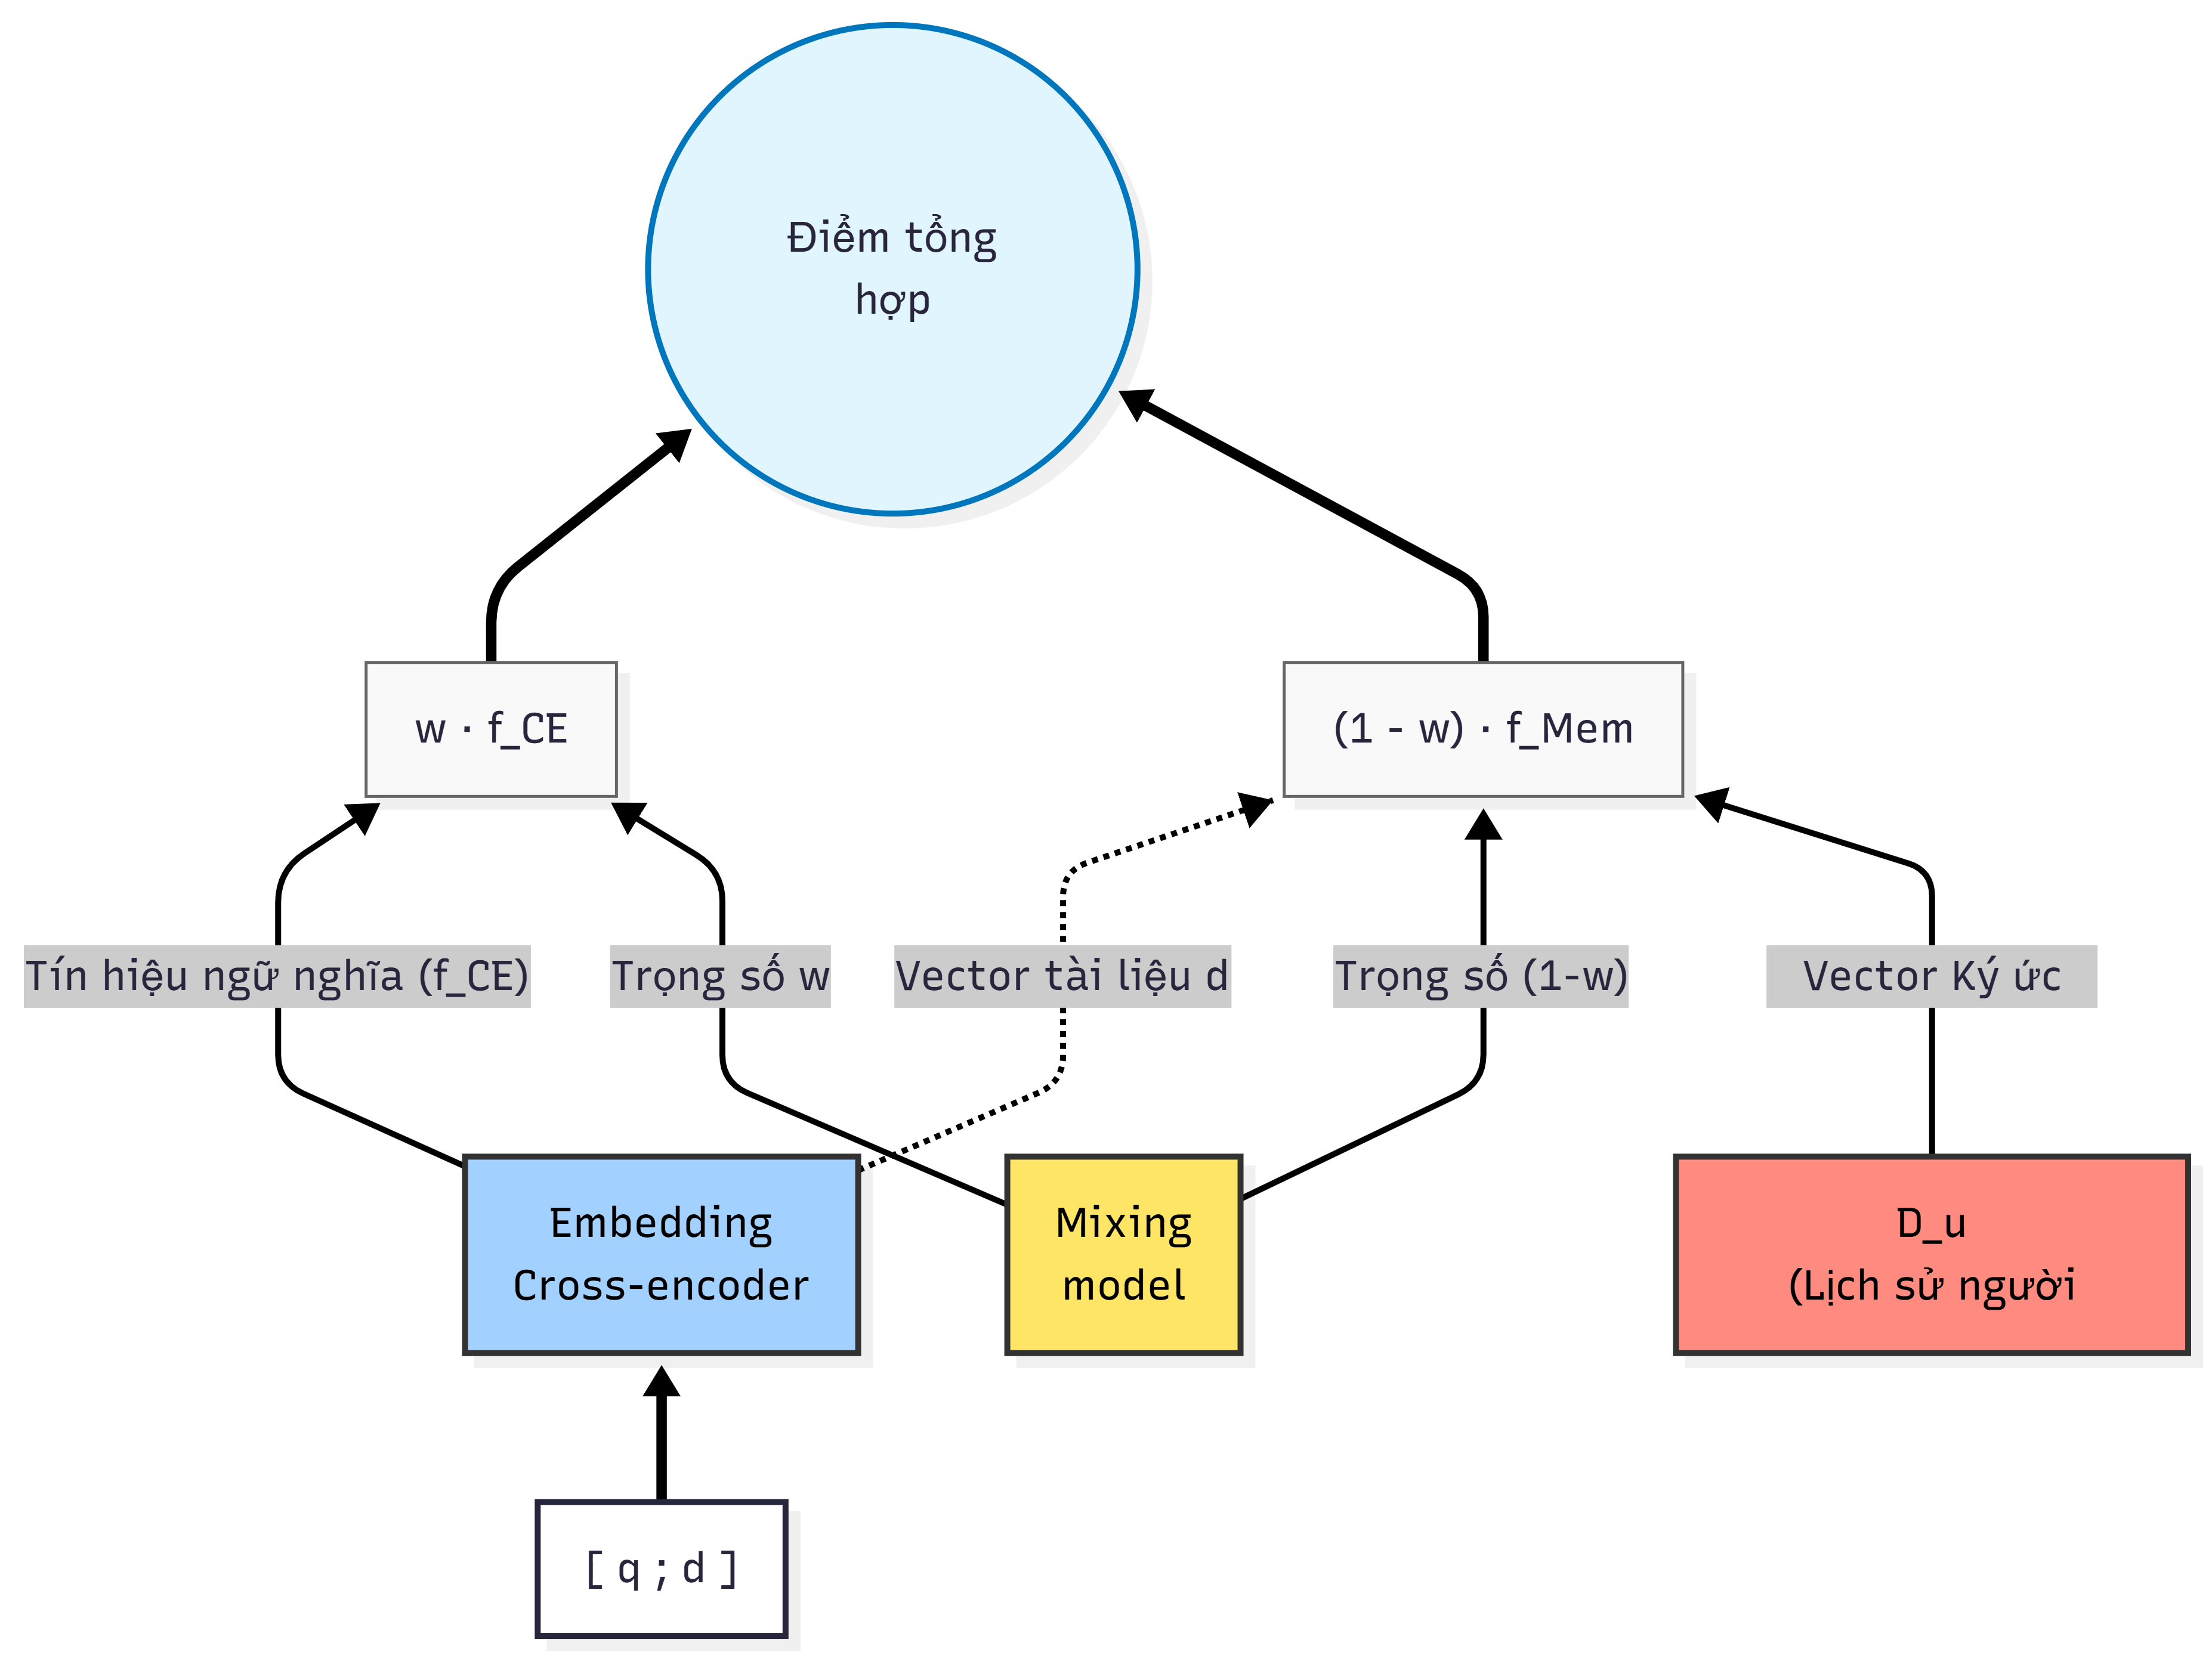
\includegraphics[width=0.85\textwidth]{Images/overview_cross_encoder.png} % Thay reranker_arch.png bằng tên file của bạn
    \vspace{0.5cm}
    \caption{Kiến trúc tổng quan của mô hình xếp hạng lại (Reranker) kết hợp đối sánh ngữ nghĩa và bộ nhớ cá nhân hóa.}
    \label{fig:reranker_arch}
\end{figure}

Sự khác biệt của kiến trúc này so với các mạng Cross-Encoder tiêu chuẩn nằm ở phương pháp biểu diễn đặc trưng. Các mô hình Cross-Encoder truyền thống thường gộp chung truy vấn và tài liệu thành một chuỗi thống nhất, làm hạn chế khả năng tách biệt và tái sử dụng đặc trưng của tài liệu cho các tác vụ khác. Ngược lại, mô hình đề xuất sử dụng kiến trúc Embedding Cross-Encoder, cho phép học các biểu diễn vector tách biệt nhưng vẫn chứa đựng thông tin ngữ cảnh chéo (cross-encoded) cho cả truy vấn ($\mathbf{q}$) và tài liệu ($\mathbf{d}$). Nhờ cấu trúc phân mảnh này, vector biểu diễn của tài liệu có thể trực tiếp tương tác với các vector đa chiều $V_i$ trong hồ sơ người dùng $\mathcal{P}_u$ thông qua thành phần $f_{Mem}$. Đồng thời, trọng số w được sinh ra đóng vai trò như một bộ dự báo hiệu suất, giúp hệ thống đánh giá mức độ tin cậy của tín hiệu từ Cross-Encoder, qua đó quyết định xem có cần sự can thiệp từ bộ nhớ cá nhân hay không. Cấu trúc phân tách điểm số này cũng cung cấp một cơ chế điều khiển thiết yếu, cho phép hệ thống dễ dàng quay về trạng thái không cá nhân hóa thông qua thao tác loại bỏ thành phần $s_d^u$ khỏi phương trình tính toán khi không cần thiết.

Tổng thể kiến trúc của giai đoạn xếp hạng lại được xây dựng theo dạng mô-đun nhằm cân bằng giữa việc phân tích ngữ nghĩa và khai thác thông tin cá nhân hóa. Cách tiếp cận này giúp hệ thống khắc phục được tính cứng nhắc của các phương pháp truyền thống, đồng thời cho phép kiểm soát linh hoạt mức độ can thiệp của dữ liệu lịch sử đối với từng truy vấn cụ thể. Thiết kế phân tách rõ ràng giữa các thành phần học ngữ nghĩa và thành phần trộn điểm cũng tạo nền tảng thuận lợi cho việc tối ưu hóa độc lập trong các quá trình huấn luyện tiếp theo.

\subsection{Embedding Cross Encoder}

Các kiến trúc Cross-Encoder tiêu chuẩn hiện đóng vai trò nền tảng trong nhiều hệ thống xếp hạng văn bản tiên tiến nhờ khả năng phân tích ngữ nghĩa sâu sắc và đánh giá mức độ liên quan với độ chính xác cao. Theo cách tiếp cận truyền thống, các mô hình này tiến hành ghép nối trực tiếp câu truy vấn và tài liệu ứng viên thành một chuỗi duy nhất thông qua các token phân cách, sau đó nạp toàn bộ chuỗi này qua các tầng tự chú ý (self-attention) của mô hình ngôn ngữ. Mặc dù phương pháp này tối ưu hóa được việc học các tương tác từ vựng chéo ở mức độ token (token-level cross-attention), nó lại bộc lộ một rào cản kiến trúc nghiêm trọng khi được tích hợp vào các hệ thống đòi hỏi tính cá nhân hóa. Nguyên nhân cốt lõi nằm ở việc các mô hình này thường nén toàn bộ thông tin của cặp truy vấn - tài liệu vào một token đại diện duy nhất (thường là token [CLS]) để tính toán ra một điểm số vô hướng cuối cùng. Sự hợp nhất này làm xóa nhòa ranh giới đặc trưng không gian của tài liệu. Khi không thể trích xuất được một biểu diễn vector độc lập đại diện cho tài liệu, hệ thống hoàn toàn thiếu đi cơ sở dữ liệu véc-tơ để tiếp tục đối chiếu với các nguồn thông tin khác, đặc biệt là không gian vector đa chiều chứa bộ nhớ về lịch sử tương tác của người dùng.

\begin{figure}[htbp]
    \centering
    % Dùng width=1\textwidth để ép hình ngang tràn viền lề, hiển thị to và rõ nhất
    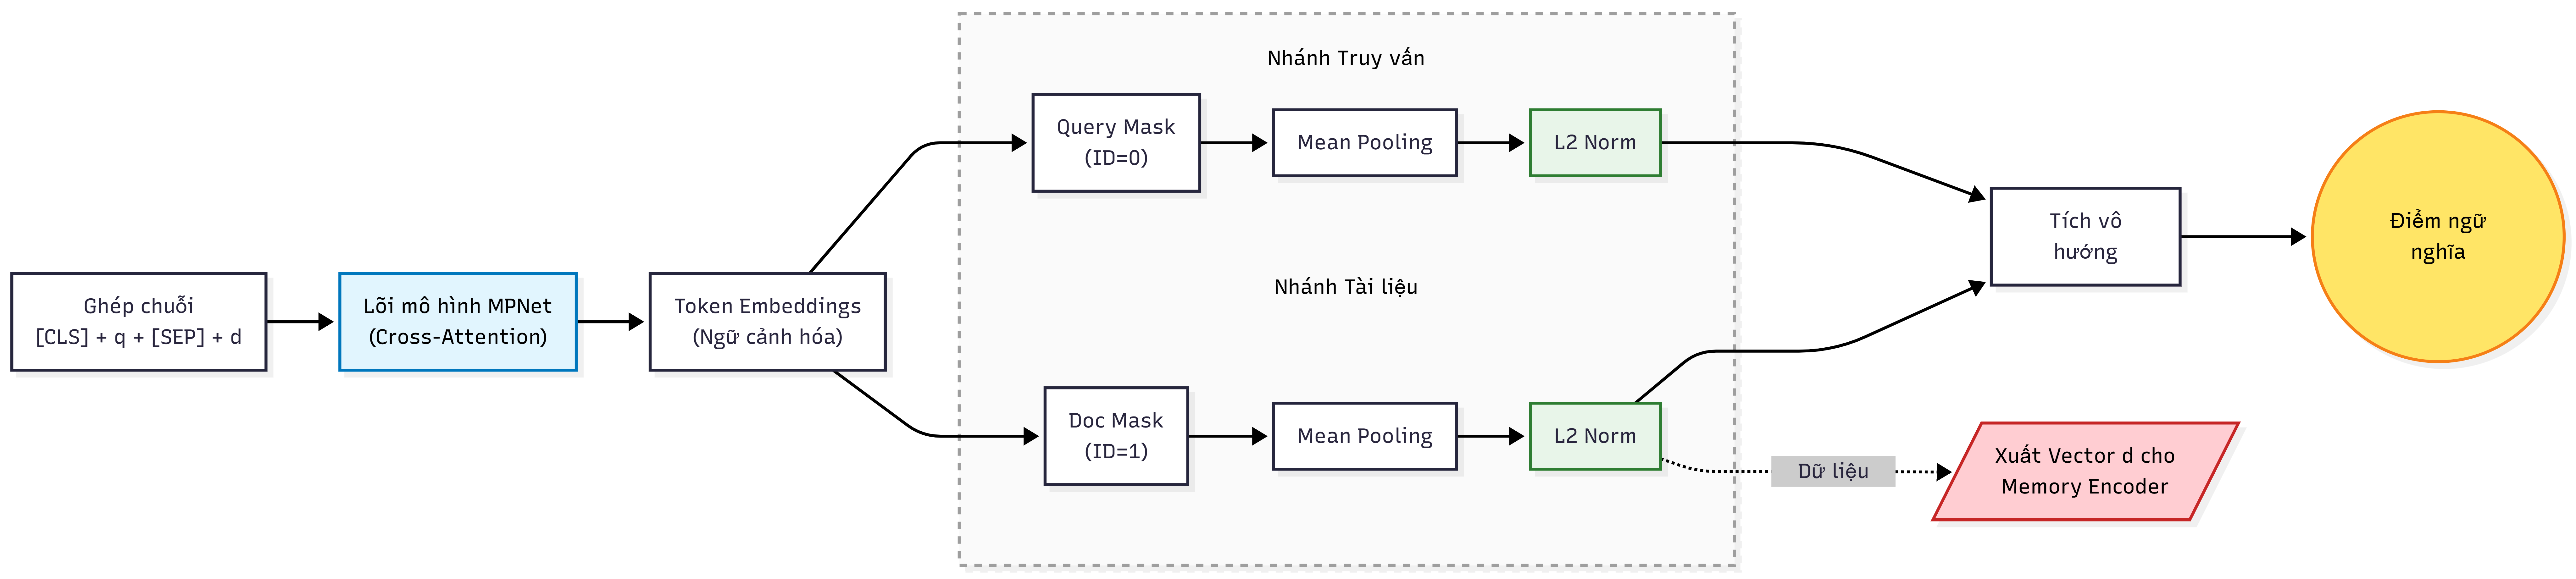
\includegraphics[width=1\textwidth]{Images/embedding_cross_encoder.png} % Thay embedding_ce.png bằng tên file của bạn
    \vspace{0.5cm}
    \caption{Sơ đồ luồng xử lý và trích xuất đặc trưng độc lập của kiến trúc Embedding Cross-Encoder.}
    \label{fig:embedding_ce}
\end{figure}

Để vượt qua giới hạn kiến trúc này, một cơ chế mang tên Embedding Cross-Encoder được triển khai, sử dụng mô hình ngôn ngữ MPNet làm lõi xử lý trung tâm. Lõi MPNet được ưu tiên lựa chọn nhờ khả năng nắm bắt ngữ nghĩa toàn cục vượt trội, bắt nguồn từ phương pháp huấn luyện kết hợp giữa cơ chế che giấu từ (masked language modeling) và hoán vị từ (permuted language modeling), giúp mô hình hiểu được cấu trúc ngữ cảnh phức tạp của các chuỗi văn bản dài. Quá trình xử lý của Embedding Cross-Encoder vẫn duy trì bước khởi đầu quen thuộc: nạp chuỗi ghép nối giữa truy vấn và tài liệu vào mô hình để trích xuất các biểu diễn token mang tính ngữ cảnh (contextualized token embeddings) từ tầng ẩn cuối cùng. Tuy nhiên, sự khác biệt mang tính đột phá nhằm giải quyết bài toán biểu diễn nằm ở bước phân tách đặc trưng. Thay vì sử dụng đầu ra từ token [CLS], hệ thống tận dụng các chuỗi định danh (sequence IDs) do bộ phân tách từ ngữ (tokenizer) cung cấp để xác định rõ ranh giới ngữ nghĩa. Dựa trên các định danh này, các ma trận mặt nạ (attention mask) chuyên biệt được tạo ra để định vị và cô lập chính xác tập hợp các token thuộc về câu truy vấn và tập hợp các token thuộc về tài liệu ứng viên. 

Ngay sau khi quá trình cô lập nhóm token hoàn tất, kỹ thuật gộp trung bình (mean pooling) được áp dụng một cách độc lập lên từng nhóm token tương ứng với mặt nạ phân bổ của chúng. Kết quả của phép toán này là sự hình thành của hai biểu diễn vector hoàn toàn tách biệt có cùng không gian số chiều: một vector đại diện cho truy vấn (q) và một vector đại diện cho tài liệu (d). Nhằm đảm bảo tính ổn định và đồng nhất trong hình học không gian vector, cả hai biểu diễn này đều tiếp tục trải qua quá trình chuẩn hóa L2 (L2 Normalization), đưa toàn bộ các giá trị về cùng một không gian độ đo chuẩn mực. Sau khi được chuẩn hóa, điểm số đánh giá mức độ phù hợp ngữ nghĩa cốt lõi giữa truy vấn và tài liệu được tính toán trực tiếp thông qua phép toán tích vô hướng của hai vector này. Nhờ sự hiện diện của bước chuẩn hóa trước đó, tích vô hướng ở công đoạn này mang ý nghĩa toán học tương đương với việc đo lường độ cosine similarity, phản ánh một cách trực quan và chính xác sự hội tụ về mặt ý nghĩa giữa ý định tìm kiếm của người dùng và nội dung cốt lõi của văn bản.

Nhìn chung, việc thiết kế và ứng dụng cơ chế Embedding Cross-Encoder mang lại những lợi ích mang tính bản lề cho toàn bộ kiến trúc của giai đoạn xếp hạng lại. Một mặt, kiến trúc này vẫn kế thừa trọn vẹn khả năng phân tích sự phụ thuộc từ vựng phức tạp nhờ cơ chế tự chú ý chéo diễn ra liên tục trong các tầng sâu của mô hình MPNet, qua đó bảo chứng cho độ chính xác cao của tín hiệu tìm kiếm ngữ nghĩa độc lập. Mặt khác, sự can thiệp mang tính cấu trúc ở lớp đầu ra đã giải phóng đặc trưng của tài liệu khỏi trạng thái nén cứng nhắc truyền thống. Vector tài liệu (d) được trích xuất ra mang một đặc tính lai độc đáo: nó vừa tồn tại như một thực thể toán học độc lập trong không gian vector, vừa chứa đựng dấu ấn ngữ cảnh sâu sắc từ sự tương tác trực tiếp với câu truy vấn. Chính biểu diễn tài liệu đã được ngữ cảnh hóa này sẽ đóng vai trò là đầu vào tiên quyết để thực hiện các phép toán đối chiếu chéo với bộ nhớ người dùng, kiến tạo nên tiền đề kỹ thuật vững chắc để hệ thống triển khai các thuật toán cá nhân hóa ở những giai đoạn tiếp theo một cách minh bạch và hiệu quả.


\subsection{Memory Encoder}

Sau khi trích xuất thành công vector biểu diễn tài liệu độc lập từ mô-đun Embedding Cross-Encoder, hệ thống tiến tới giai đoạn định lượng mức độ phù hợp của tài liệu ứng viên đối với từng người dùng cụ thể. Việc chỉ phụ thuộc vào câu truy vấn hiện tại sẽ bỏ qua nguồn thông tin ngữ cảnh có giá trị lớn ẩn chứa trong lịch sử tương tác. Tuy nhiên, lịch sử của một người dùng thường bao gồm một tập hợp nhiều sản phẩm hoặc tài liệu mang các chủ đề rất đa dạng. Do đó, việc đối chiếu trực tiếp một tài liệu mới với toàn bộ chuỗi sự kiện trong quá khứ đặt ra một thách thức lớn về mặt biểu diễn không gian. Hệ thống đòi hỏi một cơ chế tính toán chuyên biệt nhằm chuyển đổi dữ liệu lịch sử thô thành các tín hiệu cá nhân hóa có khả năng đo lường chính xác, mà không làm mất đi các sắc thái sở thích riêng biệt.

\begin{figure}[htbp]
    \centering
    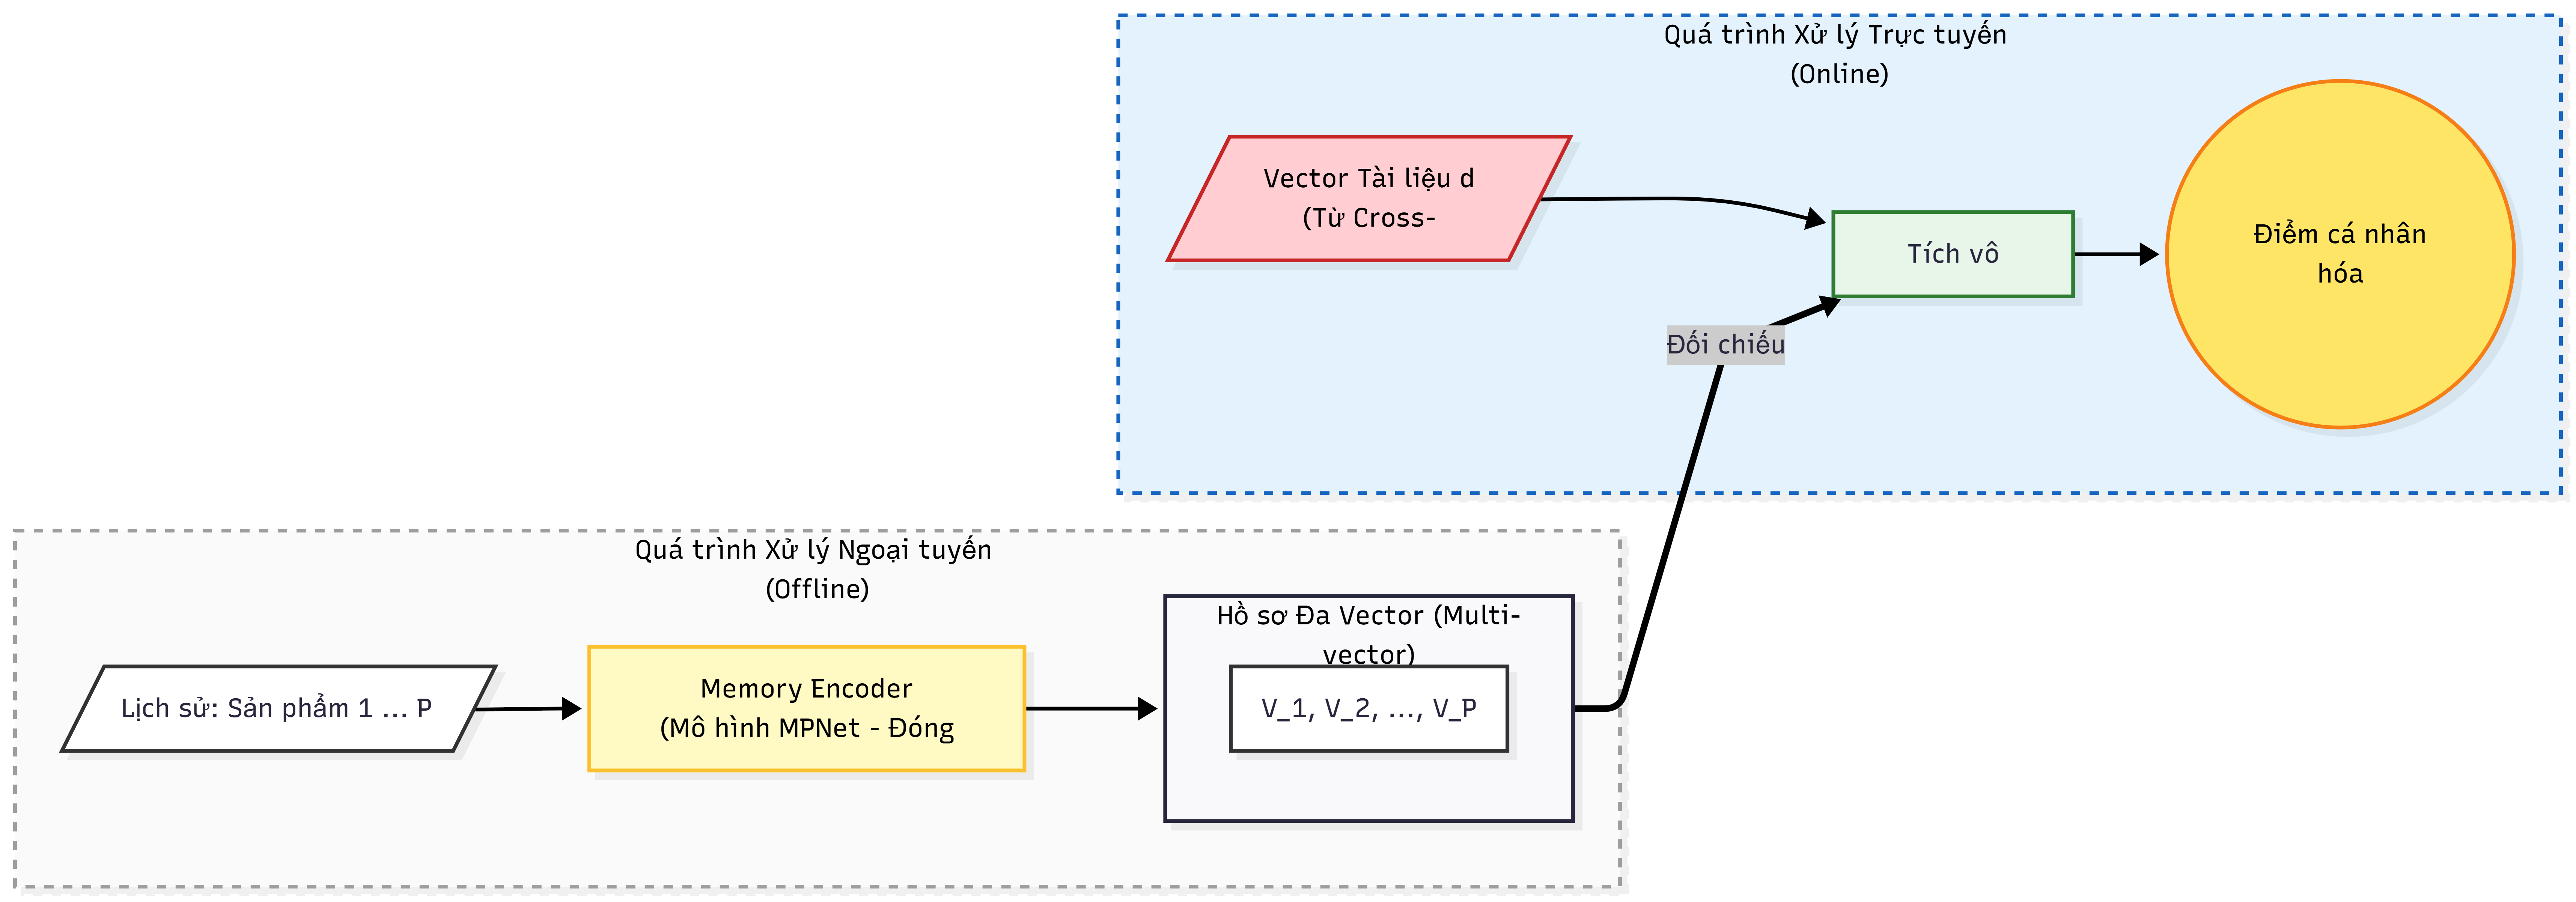
\includegraphics[width=1\textwidth]{Images/Embedding Cross-encoder-2026-04-30-153925.png} 
    \vspace{0.5cm}
    \caption{Cơ chế hoạt động của Memory Encoder phân tách thành hai luồng: Xử lý ngoại tuyến (chắt lọc hồ sơ đa vector) và Xử lý trực tuyến (đối chiếu và tính điểm cá nhân hóa).}
    \label{fig:memory_encoder}
\end{figure}

Để giải quyết bài toán này, mô-đun Memory Encoder (Bộ mã hóa ký ức) được thiết kế nhằm số hóa và quản lý hồ sơ người dùng dưới dạng một cấu trúc bộ nhớ đa vector (Multi-vector User Representation). Trong cơ chế này, lịch sử tương tác được xem như một tập hợp các tài liệu độc lập, và mỗi tài liệu cấu thành nên lịch sử đó sẽ được nạp qua một mô hình ngôn ngữ chuyên biệt nhằm tạo ra một tập hợp các vector biểu diễn ký ức ($V_i$) riêng biệt. Nhằm tối ưu hóa tài nguyên tính toán và giảm thiểu độ trễ, toàn bộ quá trình mã hóa bộ nhớ này được thực hiện ngoại tuyến (offline) với các trọng số của mô hình mã hóa được đóng băng hoàn toàn. Điểm số đánh giá mức độ cá nhân hóa ($s_d^u$) của tài liệu ứng viên được xác định dựa trên độ tương đồng vô hướng (dot product) giữa vector tài liệu mục tiêu (d) — được truyền sang từ nhánh Cross-Encoder — và từng vector ký ức trong hồ sơ người dùng. Cụ thể, hệ thống áp dụng toán tử tìm giá trị lớn nhất (max pooling) trên toàn bộ tập hợp các điểm số tương đồng vừa tính toán. Thao tác toán học này đảm bảo rằng tài liệu ứng viên chỉ cần có độ cộng hưởng mạnh mẽ với một phần sở thích cốt lõi trong quá khứ là đủ để ghi nhận điểm cá nhân hóa cao, ngăn chặn hiện tượng các tín hiệu nổi bật bị làm loãng nếu áp dụng các phép tính trung bình hóa thông thường.

Nhìn chung, Memory Encoder đóng vai trò như một bộ lọc cá nhân hóa có độ phân giải cao trong tổng thể kiến trúc xếp hạng lại. Bằng cách duy trì trực tiếp các biểu diễn vector độc lập của từng sản phẩm thay vì nén toàn bộ lịch sử thành một khối dữ liệu duy nhất, kiến trúc này bảo toàn trọn vẹn các đặc trưng chi tiết trong sở thích của người dùng. Tín hiệu cá nhân hóa độc lập và sắc bén được sinh ra từ mô-đun này không chỉ phản ánh mức độ thân thuộc của tài liệu ứng viên, mà còn cung cấp một tham chiếu định lượng thiết yếu. Đây chính là mảnh ghép dữ liệu hoàn chỉnh giúp bộ trộn ở công đoạn tiếp theo có khả năng cân đối một cách linh hoạt giữa kết quả đối sánh ngữ nghĩa và thói quen tương tác dài hạn của người dùng.


\subsection{Mixing Model}

Trong các hệ thống tìm kiếm kết hợp (hybrid search), việc trích xuất thành công hai nguồn điểm số độc lập đại diện cho độ phù hợp ngữ nghĩa và độ phù hợp cá nhân hóa mới chỉ là bước khởi đầu. Thách thức kiến trúc lớn nhất ở giai đoạn dung hợp đặc trưng nằm ở hiện tượng mất cân bằng tín hiệu, thường được nhắc đến trong lý thuyết học máy là sự sụp đổ phương thức (modality collapse) hoặc vấn đề áp đảo (dominance problem). Trên thực tế, mức độ cần thiết của thông tin cá nhân hóa biến thiên rất lớn tùy thuộc vào bản chất của từng phiên tìm kiếm: các truy vấn mang tính khám phá hoặc đa nghĩa đòi hỏi sự định hướng mạnh mẽ từ hồ sơ người dùng, trong khi các truy vấn tra cứu định danh cụ thể lại chỉ cần đối sánh từ vựng chính xác. Nếu hệ thống áp dụng một phương pháp kết hợp tuyến tính với trọng số cố định hoặc nội suy đơn giản, mô hình thường có xu hướng hội tụ về trạng thái mất cân đối, nơi nó chỉ phụ thuộc vào tín hiệu dễ học và triệt tiêu hoàn toàn vai trò của bộ nhớ lịch sử.

Nhằm khắc phục triệt để điểm yếu kiến trúc này, một mô hình trộn động (Mixing Model, ký hiệu là $g_{Mix}$) được thiết kế để điều phối toàn bộ quá trình tính toán kết quả từ các đầu vào cơ sở: câu truy vấn (q), tài liệu ứng viên (d) và hồ sơ lịch sử người dùng ($\mathcal{P}_u$). Về mặt toán học, điểm số xếp hạng cuối cùng ($s_d$) của một tài liệu được xác định thông qua phương trình nội suy kết hợp giữa tích vô hướng của các vector ngữ nghĩa và phép toán tìm cực đại trên không gian bộ nhớ:

$$s_d = w \cdot \mathbf{q}^T \mathbf{d} + (1-w) \cdot \max_{i \in \{1...P\}} \mathbf{d}^T \mathbf{V}_i$$

Trong đó, $\mathbf{q}^T \mathbf{d}$ chính là điểm phù hợp ngữ nghĩa ($s_d^q$) do Embedding Cross-Encoder trích xuất, và $\max \mathbf{d}^T \mathbf{V}_i$ là điểm cá nhân hóa ($s_d^u$) được đối chiếu từ P vector ký ức trong Memory Encoder. Trọng tâm của sự linh hoạt nằm ở việc xác định trọng số điều phối w. Thay vì gán một giá trị tĩnh, trọng số này được dự đoán liên tục thông qua một mạng nơ-ron đa tầng (MLP) kết hợp với hàm kích hoạt sigmoid nhằm giới hạn biên độ đầu ra trong khoảng [0, 1]:

$$w = \text{sigmoid}(\text{MLP}([\mathbf{q}, len(q), P, s_d^q, s_d^u]))$$

Đầu vào của mạng MLP này không chỉ dừng lại ở hai điểm số thành phần ($s_d^q$ và $s_d^u$), mà còn bao gồm một tập hợp các đặc trưng ngữ cảnh (metadata) mang tính quyết định: vector biểu diễn gốc của truy vấn ($\mathbf{q}$), độ dài của chuỗi truy vấn (len(q)), và quy mô cấu trúc của bộ nhớ người dùng (P).

Sự tích hợp của mô hình trộn động đã biến kiến trúc xếp hạng từ một cỗ máy tính toán tĩnh thành một hệ thống thích ứng ngữ cảnh mang tính dự báo. Về bản chất, thành phần này vận hành như một bộ dự báo hiệu suất (performance predictor): bằng cách phân tích hình thái của câu truy vấn và độ phong phú của dữ liệu lịch sử, nó tự động đánh giá mức độ tin cậy của nhánh đối sánh ngữ nghĩa để từ đó đưa ra quyết định cấp phát trọng số tương ứng cho nhánh cá nhân hóa. Cơ chế điều tiết tinh vi này không những giải quyết thành công bài toán áp đảo phương thức mà còn đảm bảo sự dung hòa tuyệt đối giữa ý định tìm kiếm tức thời và thói quen tiêu dùng dài hạn, cho phép hệ thống cung cấp các kết quả tìm kiếm được cá nhân hóa một cách chừng mực và tự nhiên nhất.

\subsection{Chiến thuật Huấn luyện}

\subsubsection*{Khởi tạo và thiết lập mô hình}

Quá trình huấn luyện đồng thời (end-to-end) toàn bộ kiến trúc kết hợp giữa đối sánh ngữ nghĩa và cá nhân hóa thường dẫn đến hiện tượng nhiễu loạn gradient. Sự giao thoa của các luồng tín hiệu cập nhật trọng số khác biệt có thể làm suy giảm nghiêm trọng khả năng biểu diễn ngôn ngữ cốt lõi của hệ thống. Để giải quyết rào cản này, một chiến lược huấn luyện phân tách (decoupled training) được triển khai, chia quá trình tối ưu hóa thành hai giai đoạn độc lập. Đi kèm với đó là các thiết lập khởi tạo chuyên biệt cho từng bộ mã hóa trên tập dữ liệu thương mại điện tử Amazon Review nhằm tận dụng tối đa tri thức ngôn ngữ từ các mô hình học sâu tiên tiến.

Đối với nhánh mã hóa chéo ($Enc_{CE}$), hệ thống không khởi tạo trọng số ngẫu nhiên mà kế thừa trực tiếp từ kiến trúc tiền huấn luyện \texttt{sentence-transformers/all-mpnet-base-v2}. Việc lựa chọn phiên bản này xuất phát từ hai lý do cốt lõi. Thứ nhất, về mặt nền tảng, nó vẫn kế thừa trọn vẹn kiến trúc MPNet cơ sở với khả năng tổng hợp ưu điểm của hai phương pháp học ngôn ngữ hàng đầu: cơ chế che giấu từ (Masked Language Modeling - MLM) giúp nắm bắt cấu trúc từ vựng cục bộ, và cơ chế hoán vị từ (Permuted Language Modeling - PLM) giúp hiểu được sự phụ thuộc ngữ cảnh toàn cục. Thứ hai, phiên bản \texttt{all-mpnet-base-v2} đã trải qua quá trình tối ưu hóa đặc biệt trên một bộ dữ liệu quy mô lớn gồm hơn 1 tỷ cặp câu, cung cấp một không gian vector biểu diễn tổng quát (sentence embeddings) có độ chính xác rất cao. Sau khi được khởi tạo với nền tảng trọng số mạnh mẽ này, lõi mô hình tiếp tục được tinh chỉnh (fine-tune) trực tiếp trên kho ngữ liệu của tập dữ liệu Amazon Review. Thao tác này mang ý nghĩa tiên quyết giúp mô hình làm quen với các thuật ngữ chuyên ngành, sự phân bố từ vựng đặc thù và các dạng tương tác từ vựng chéo phổ biến trong miền thương mại điện tử.

Ngược lại, đối với nhánh mã hóa ký ức ($Enc_{Mem}$), hệ thống tái sử dụng trọng số từ mô hình tiền huấn luyện \texttt{sentence-transformers/multi-qa-mpnet-base-cos-v1}. Đây là một biến thể của kiến trúc MPNet đã được tinh chỉnh chuyên sâu để tối ưu hóa cho các tác vụ hỏi đáp và truy xuất thông tin dày đặc (dense retrieval) dựa trên độ đo tương đồng cosine. Nhằm đảm bảo hệ thống có thể hoạt động trơn tru và mở rộng quy mô trên các phần cứng GPU tiêu chuẩn mà không gặp hiện tượng tràn bộ nhớ, toàn bộ hệ số trọng lượng của nhánh $Enc_{Mem}$ được đóng băng (frozen) ngay từ đầu. Chiến lược đóng băng này cho phép hệ thống thực hiện trích xuất và tính toán trước toàn bộ không gian bộ nhớ của người dùng ($\mathcal{P}_u$) một cách ngoại tuyến (offline), giúp tiết kiệm đáng kể dung lượng bộ nhớ và tài nguyên tính toán cho các công đoạn tối ưu hóa phía sau.

\subsubsection*{Giai đoạn 2 (Phase 2): Huấn luyện điều chuẩn $g_{Mix}$}

Giai đoạn huấn luyện đầu tiên được thiết kế với mục tiêu duy nhất là tối ưu hóa khả năng phân tích và trích xuất điểm số phù hợp ngữ nghĩa ($s_d^q$) của mô-đun $Enc_{CE}$ từ các cặp truy vấn và tài liệu ứng viên. Trong toàn bộ pha này, mô hình trộn cùng với điểm số cá nhân hóa hoàn toàn bị loại bỏ khỏi luồng tính toán. Sự cô lập này ép buộc nhánh mã hóa chéo phải tự mình học cách phân biệt sự liên quan ngữ nghĩa một cách khách quan nhất mà không có bất kỳ sự định hướng nào từ thông tin hồ sơ lịch sử.

Để đạt được mục tiêu tối ưu hóa, hệ thống áp dụng khung học tương phản (contrastive learning) làm nguyên lý cấu trúc dữ liệu cốt lõi. Cụ thể, đối với mỗi truy vấn q được trích xuất từ tập huấn luyện, dữ liệu đầu vào sẽ bao gồm một tài liệu tích cực đích thực (đại diện cho kết quả khớp chuẩn) đi kèm với một tập hợp gồm M tài liệu tiêu cực đóng vai trò là mồi nhử (negative samples). Tập dữ liệu ghép nối này sau khi đi qua quá trình mã hóa sẽ sinh ra một vector điểm số dự đoán liên tục, ký hiệu là $s_q$, tương ứng với một vector nhãn gốc $y_q$ mang giá trị phân phối nhị phân (trong đó duy nhất vị trí của tài liệu tích cực nhận giá trị 1, các mồi nhử còn lại nhận giá trị 0).

Quá trình cập nhật trọng số của mạng nơ-ron được dẫn dắt trực tiếp bởi hàm mất mát Softmax Cross-Entropy tiêu chuẩn. Việc áp dụng hàm loss này trên một tập hợp bao gồm cả mẫu tích cực và các mẫu tiêu cực nội lô (in-batch negatives) đã được chứng minh là phương pháp cốt lõi mang lại hiệu suất vượt trội cho các hệ thống truy xuất văn bản hiện đại \cite{22}. Về mặt toán học, hàm mất mát Softmax Cross-Entropy tiêu chuẩn \cite{22} được biểu diễn thông qua phương trình:
$$\mathcal{L}(y_q, s_q) = - \sum_{i=1}^M y_q[i] \log \text{sm}(s_q[i])$$

Trong phương trình trên, toán tử sm đại diện cho hàm phân phối xác suất softmax. Việc tối thiểu hóa hàm $\mathcal{L}$ mang một ý nghĩa hình học rõ ràng: nó tạo ra một lực đẩy ép mô hình $Enc_{CE}$ phải điều chỉnh không gian vector biểu diễn sao cho điểm số $s_d^q$ của tài liệu tích cực luôn được khuếch đại, từ đó áp đảo hoàn toàn xác suất của hàng loạt tài liệu nhiễu trong cùng một không gian đối chiếu. Kết thúc giai đoạn này, nhánh ngữ nghĩa đã đạt trạng thái sẵn sàng cao nhất để làm nền tảng cho việc dung hợp thông tin cá nhân hóa ở pha tiếp theo.

\subsubsection*{Giai đoạn 2 (Phase 2): Huấn luyện điều chuẩn $g_{Mix}$}

\textbf{Mục tiêu và Tích hợp tham số tỷ lệ:}
Bước sang giai đoạn thứ hai, trọng số của cả hai nhánh mã hóa $Enc_{CE}$ và $Enc_{Mem}$ đều được đóng băng cố định nhằm bảo toàn trọn vẹn không gian biểu diễn đã được thiết lập ở pha trước. Mục tiêu cốt lõi lúc này là tập trung huấn luyện mạng nơ-ron đa tầng của mô hình trộn $g_{Mix}$ học cách dự đoán chính xác trọng số điều phối w. Trọng số này đóng vai trò quyết định trong việc thiết lập tỷ lệ nội suy giữa điểm phù hợp ngữ nghĩa ($s_d^q$) và điểm cá nhân hóa ($s_d^u$). Điểm đáng chú ý mang tính đột phá trong kiến trúc tối ưu hóa của pha này là sự tích hợp của một tham số tỷ lệ có khả năng học (learnable scale parameter), được thiết kế lấy cảm hứng từ các mô hình mạng nơ-ron đối chiếu tiên tiến (như kiến trúc CLIP). Tham số này được khởi tạo với giá trị logarit tương đương tỷ lệ 1/0.07 (xấp xỉ 14.3) và không bị khóa cứng; ngược lại, nó được mô hình tự động tinh chỉnh linh hoạt trong suốt quá trình huấn luyện nhằm kiểm soát độ nhạy (temperature) của dải điểm số đầu ra trước khi đưa vào hàm tính toán xác suất.

\textbf{Cấu trúc dữ liệu và Mỏ neo:}
Về mặt cấu trúc dữ liệu, Giai đoạn 2 tiếp tục kế thừa nguyên vẹn tập hợp dữ liệu gồm một mẫu tích cực và M mẫu tiêu cực. Tuy nhiên, hệ thống chèn thêm một điểm mỏ neo (anchor) nhân tạo vào tập điểm số với logit mục tiêu cố định $s_0 = 0$, đi kèm với nhãn mục tiêu điều chỉnh là $y_0$ (đóng vai trò là một siêu tham số). Sự can thiệp có chủ đích này, khi được kết hợp với phép nhân vô hướng từ tham số tỷ lệ (logit scale) liên tục cập nhật, sẽ tự động khuếch đại hoặc thu hẹp khoảng cách tương đối giữa các giá trị dự đoán, từ đó biến đổi vector điểm số thô ban đầu thành $s'_q$ và vector nhãn tương ứng thành $y'_q$.

\textbf{Hàm mất mát và Ý nghĩa hiệu chuẩn:}
Để ngăn chặn tình trạng mạng MLP sinh ra các dự đoán quá tự tin (overconfident predictions) dẫn đến hiện tượng sụp đổ phương thức (modality collapse), hệ thống từ bỏ hàm Softmax tiêu chuẩn và thay thế bằng hàm Scale Calibrating Softmax Objective \cite{30}:

$$ \mathcal{L}(y'_q, s'_q) = - \sum_{i=1}^M y'_q[i] \log \frac{e^{s'_q[i]}}{\sum_j e^{s'_q[j]} + 1} + y_0 \log \left( \sum_j e^{s'_q[j]} + 1 \right) $$

Việc chèn biến neo $y_0$ vào hàm loss đóng vai trò như một cơ chế chính quy hóa (regularization) mang tính cấu trúc. Cụ thể, thành phần thứ hai của phương trình tạo ra một lực phạt nghiêm ngặt đối với các điểm số dự đoán quá lớn, trong khi thành phần thứ nhất đảm bảo các điểm số nhỏ không bị tiêu biến hoàn toàn. Dưới sự điều tiết kép của hàm loss hiệu chuẩn và tham số tỷ lệ (logit scale), trọng số w do $g_{Mix}$ sinh ra sẽ không bị cực đoan hóa về các thái cực tuyệt đối 0 hoặc 1. Thay vào đó, nó biến thiên một cách mượt mà, bám sát và phản chiếu đúng mức độ tin cậy thực tế của nhánh ngữ nghĩa, cho phép hệ thống tìm kiếm hòa trộn các tín hiệu cá nhân hóa một cách tự nhiên, chừng mực và đạt độ ổn định cao nhất.









\section{Tích hợp LLM trong Giai đoạn Hậu Truy xuất}

Trong kiến trúc tổng thể của hệ thống, Mô hình Ngôn ngữ Lớn Google Gemini được tích hợp vào giai đoạn hậu truy xuất (\textit{Post-Retrieval Stage}). Trong khi mô hình Two-Tower đóng vai trò bộ lọc thô (\textit{Coarse Filter}) giúp truy xuất nhanh các ứng viên tiềm năng dựa trên độ tương đồng vector, thì mô-đun LLM đảm nhận chức năng bộ lọc tinh và tác nhân giải thích (\textit{Explainable Agent}). Thành phần này tận dụng khả năng suy luận ngôn ngữ tự nhiên để cá nhân hóa trải nghiệm người dùng một cách sâu sắc hơn.

\subsection{Quy trình Xử lý Dữ liệu}
Quy trình tích hợp được thực hiện theo cơ chế suy luận trực tuyến (\textit{Online Inference}) thông qua bốn bước xử lý tuần tự:

\begin{enumerate}
    \item \textbf{Truy xuất Ứng viên:} \\
    Đầu vào của mô-đun là danh sách Top-$K$ sản phẩm được trả về từ mô hình Two-Tower. Tại giai đoạn này, các sản phẩm mới chỉ được định danh đơn giản bằng mã ID và điểm số tương đồng vector.
    
    \item \textbf{Làm giàu Ngữ cảnh:} \\
    Kế đến, hệ thống thực hiện các truy vấn cơ sở dữ liệu để chuyển đổi các ID vô hướng thành thông tin văn bản mang ý nghĩa ngữ nghĩa. Cụ thể:
    \begin{itemize}
        \item \textbf{Thông tin sản phẩm:} Hệ thống thu thập tiêu đề, mô tả ngắn, thông số kỹ thuật và giá tiền.
        \item \textbf{Hồ sơ người dùng:} Hệ thống truy xuất chuỗi lịch sử tương tác gần nhất, bao gồm các sản phẩm đã xem, đã mua hoặc được đánh giá cao.
    \end{itemize}
    
    \item \textbf{Kỹ thuật Prompt Engineering:} \\
    Dữ liệu sau khi làm giàu được đưa vào một khuôn mẫu cấu trúc sẵn, thiết kế theo phương pháp \textit{Zero-shot} hoặc \textit{Few-shot}. Cấu trúc này bao gồm ba thành phần chính: định nghĩa vai trò của Gemini là một chuyên gia tư vấn, cung cấp dữ liệu ngữ cảnh (lịch sử người dùng, danh sách ứng viên), và cuối cùng là nhiệm vụ yêu cầu LLM phân tích mối liên hệ sở thích để chọn lọc sản phẩm phù hợp nhất kèm theo giải thích.
    
    \item \textbf{Sinh Phản hồi:} \\
    Cuối cùng, Prompt hoàn chỉnh được gửi đến API của Gemini. Kết quả trả về là văn bản tự nhiên, sau đó được hệ thống phân tích (parse) để hiển thị lên giao diện Web Demo dưới dạng danh sách gợi ý đi kèm lời bình chi tiết.
\end{enumerate}

\subsection{Cấu trúc Prompt Minh họa}
Để LLM thực hiện tác vụ chọn lọc và giải thích mà không cần áp dụng thuật toán xếp hạng lại phức tạp, nhóm nghiên cứu sử dụng cấu trúc Prompt định hướng ngữ nghĩa như sau:

\begin{center}
\fbox{
    \begin{minipage}{0.95\textwidth}
        \setlength{\parskip}{0.5em} % Tăng khoảng cách đoạn văn trong hộp
        \textbf{System Instruction:} Bạn là một trợ lý AI chuyên nghiệp trong lĩnh vực thương mại điện tử.
        
        \textbf{User Context:} Người dùng này quan tâm đến [Danh sách lịch sử: iPhone 13, Ốp lưng MagSafe, Cáp sạc Type-C].
        
        \textbf{Candidate Items:} Dưới đây là danh sách sản phẩm tiềm năng:
        \begin{itemize}
            % Bỏ ngoặc vuông [], đưa ID ra ngoài và in đậm
            \item \textbf{ID: 101} Tai nghe AirPods Pro (Chống ồn, Apple Ecosystem)
            \item \textbf{ID: 102} Nồi cơm điện Sharp (1.8L, Nấu nhanh)
            \item \textbf{ID: 103} Sạc dự phòng Anker (20000mAh, Sạc nhanh)
        \end{itemize}
        
        \textbf{Instruction:} Dựa trên lịch sử quan tâm, hãy chọn ra các sản phẩm liên quan nhất từ danh sách ứng viên. Với mỗi sản phẩm được chọn, hãy viết một câu giải thích ngắn gọn, thuyết phục, chỉ ra mối liên hệ với sở thích cũ của họ.
    \end{minipage}
}
\end{center}

\subsection{Vai trò của LLM trong Hệ thống}
Trong cấu hình hiện tại, LLM không thay đổi thứ tự xếp hạng dựa trên điểm số mà hoạt động như một lớp hậu xử lý định tính (\textit{Qualitative Post-processing}). Cơ chế này giúp khắc phục điểm yếu hộp đen của mô hình Two-Tower bằng cách minh bạch hóa lý do gợi ý. Việc cung cấp thông tin giải thích giúp người dùng hiểu rõ sự phù hợp của sản phẩm, từ đó gia tăng niềm tin và cải thiện tỷ lệ chuyển đổi (\textit{Click-through Rate}) trên hệ thống.